\documentclass[mathserif,12pt]{beamer}
 
\mode<presentation>
{
%\usetheme{CambridgeUS}
\usetheme{Boadilla}
%\usecolortheme{whale}
%\usecolortheme{seahorse} % light blue 
%\usecolortheme{whale} % dark blue
%\usecolortheme{dolphin} %blue and black
\beamertemplatenavigationsymbolsempty
%\setbeamercovered{transparent}
\setbeamercovered{invisible}
\setbeamertemplate{itemize items}[default]
\setbeamertemplate{enumerate items}[default]
%\setbeamertemplate{footline}[frame number]{}
\setbeamertemplate{footline}{%
  \raisebox{5pt}{\makebox[\paperwidth]{\hfill\makebox[10pt]{\scriptsize\insertframenumber}}}}
}

\newcommand\blfootnote[1]{%
  \begingroup
  \renewcommand\thefootnote{}\footnote{#1}%
  \addtocounter{footnote}{-1}%
  \endgroup
}

%\setbeamercovered{dynamic}

%\usepackage[english]{babel}
%\usepackage[latin1]{inputenc}
\usepackage{tikz}
% \usetikzlibrary{fadings,shapes.arrows,shadows,arrows} 
% \usetikzlibrary{decorations.text}
\usepackage{xcolor}
\definecolor{brown}{RGB}{123,50,148}
\definecolor{darkgreen}{RGB}{0,100,0}

% \usepackage{dcolumn}
% \usepackage{transparent}
% font definitions, try \usepackage{ae} instead of the following
% three lines if you don't like this look
\usepackage{mathptmx}
\usepackage[scaled=.90]{helvet}

% \usepackage{courier}
% \usepackage{latexsym}
% \usepackage{multirow} 
% \usepackage{fancybox}
\usepackage{xspace}
%\usepackage{color}
% \usepackage{wrapfig}
% \usepackage{graphicx}
% \usepackage{epsfig}
% \usepackage{fancyhdr}
% \usepackage{natbib}
% \bibliographystyle{apalike}
% \usepackage[T1]{fontenc}
% \usepackage{amsmath}
% \usepackage{mathtools}
% \usepackage{subfloat}
% \usepackage{subfig}
% \usepackage{rotating}
% \usepackage[export]{adjustbox}
\usepackage{booktabs}

\usepackage{algorithmic}

\usepackage{xkeyval}
\usepackage{xargs} % commandx 
\usepackage{todonotes}
%\usepackage{marginnote}
\usepackage{xspace}
\presetkeys{todonotes}{inline}{}
%\newcommandx{\todoir}[2][1=]{\todo[inline]{SR: #2}\xspace}
%\newcommandx{\todor}[2][1=]{\todo[linecolor=red,backgroundcolor=red!25,bordercolor=red,#1]{SR: #2}\xspace}

\usepackage{pifont} % for checkmark and xmark
\newcommand{\cmark}{\ding{51}}%
\newcommand{\xmark}{\ding{55}}%

%\usepackage[labelformat=empty]{caption}
\setbeamertemplate{caption}{\raggedright\insertcaption\par}

% \usepackage{graphics}
\usepackage{amsbsy,amsfonts}

%\usepackage{lmodern}
%\usefonttheme[onlymath]{serif}
%\newcommand{\etal}{\textit{et al.\ }}

\newcommand \ignore[1]{}
\newcommand \siva[1]{} 
\newcommand \denot[2]{[\![#1]\!]_\mathit{#2}}
%\newcommand{\argmax}[1]{\arg\underset{#1}{\max}\;}
\newcommand{\argmax}{\operatornamewithlimits{arg\,max}}
\newcommand \kcaz{\textsc{kcaz13}\xspace}
\newcommand \psempre{\textsc{ParaSempre}\xspace}
\newcommand \mwg{\textsc{mwg}\xspace}
\newcommand{\word}[1]{\textsl{#1}}        % mention of word
\newcommand{\hlight}[1]{{\color{blue!80} #1}}

\newcommand \gp{\textsc{GraphParser}\xspace}
\newcommand \free{Free917\xspace}
\newcommand \webq{WebQuestions\xspace}
\newcommand \deplambda{\textsc{DepLambda}\xspace}
\newcommand \deptree{\textsc{DepTree}\xspace}
\newcommand \simplegraph{\textsc{SimpleGraph}\xspace}
\newcommand \ccggraph{\textsc{CCGGraph}\xspace}
\newcommand \deplambdap{DepLambda+\xspace}
\newcommand \clue{\textsc{ClueWeb09}\xspace}
\newcommand \contract{\textsc{contract}\xspace}
\newcommand \expand{\textsc{expand}\xspace}


\newcommand\vect[1]{\overrightarrow{\mathbf{#1}}}
\newcommand\type[1]{\textbf{\textsc{type}}[#1]\xspace}

\renewcommand{\l}{\lambda}
\newcommand{\lx}{\lambda x }
\newcommand{\ly}{\lambda y }
\newcommand{\lz}{\lambda z }
\newcommand{\lxy}{\lx \ly}
\newcommand{\lf}{\lambda f .}
\renewcommand{\lg}{\lambda g .}
\newcommand{\fo}{f_1}
\newcommand{\ft}{f_2}
\newcommand{\ftt}{f_3}
\newcommand{\lfo}{\lambda \fo }
\newcommand{\lft}{\lambda \ft }
\newcommand{\lftt}{\lambda \ftt }
\renewcommand{\le}{\lambda e }
\newcommand{\und}{$\_$}

\newcommand{\ex}{\exists x }
\newcommand{\ey}{\exists y }
\newcommand{\ez}{\exists z }
\newcommand{\exy}{\lx \ly}
\newcommand{\ef}{\exists f }
\newcommand{\efo}{\exists \fo }
\newcommand{\et}{\exists \ft }
\newcommand{\eftt}{\exists \ftt }

\newcommand{\itype}{{\bf Ind}}
\newcommand{\etype}{{\bf Event}}
\newcommand{\ptype}{\itype \times \etype}
\newcommand{\ftype}{\eta}
\newcommand{\btype}{{\bf Bool}}
\renewcommand{\land}{\wedge}
\newcommand{\true}{\lambda x \lspace \textsc{true}}
\newcommand{\lspace}{.\,}
\newcommand{\bind}{\textsc{bind}}
\newcommand{\eqop}{\textsc{eq}}

\title[\tiny Towards a Compositional Typed Semantics for Universal Dependencies]{Towards a Compositional Typed Semantics for Universal Dependencies}

\vspace{-2cm}
\author[]{\small Siva Reddy}

\institute{
\vspace{-0.5cm}

School of Informatics\\The University of Edinburgh\\
}
  
% \date{}
\date[]{}

\begin{document}

\begin{frame}
\titlepage

% \begin{center}
% NAACL 2016
% \end{center}
\end{frame}

\begin{frame}
\frametitle{People}
  \begin{center}
\begin{tabular}{c c c c}
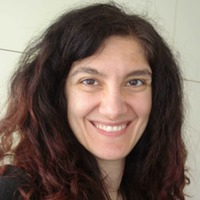
\includegraphics[width=1.5cm]{figures/mirella} & 
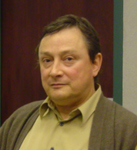
\includegraphics[width=1.5cm]{figures/steedman} &
\visible<2->{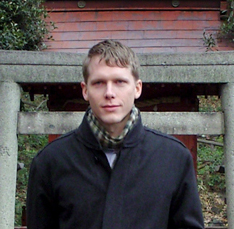
\includegraphics[width=1.5cm]{figures/oscar} &
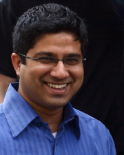
\includegraphics[width=1.2cm]{figures/dipanjan}} \\
\footnotesize Mirella~Lapata & \footnotesize Mark~Steedman & \visible<2->{\footnotesize Oscar~T\"ackstr\"om & \footnotesize Dipanjan Das} \\
\\
\end{tabular}

\visible<2->{
\begin{tabular}{c c c}
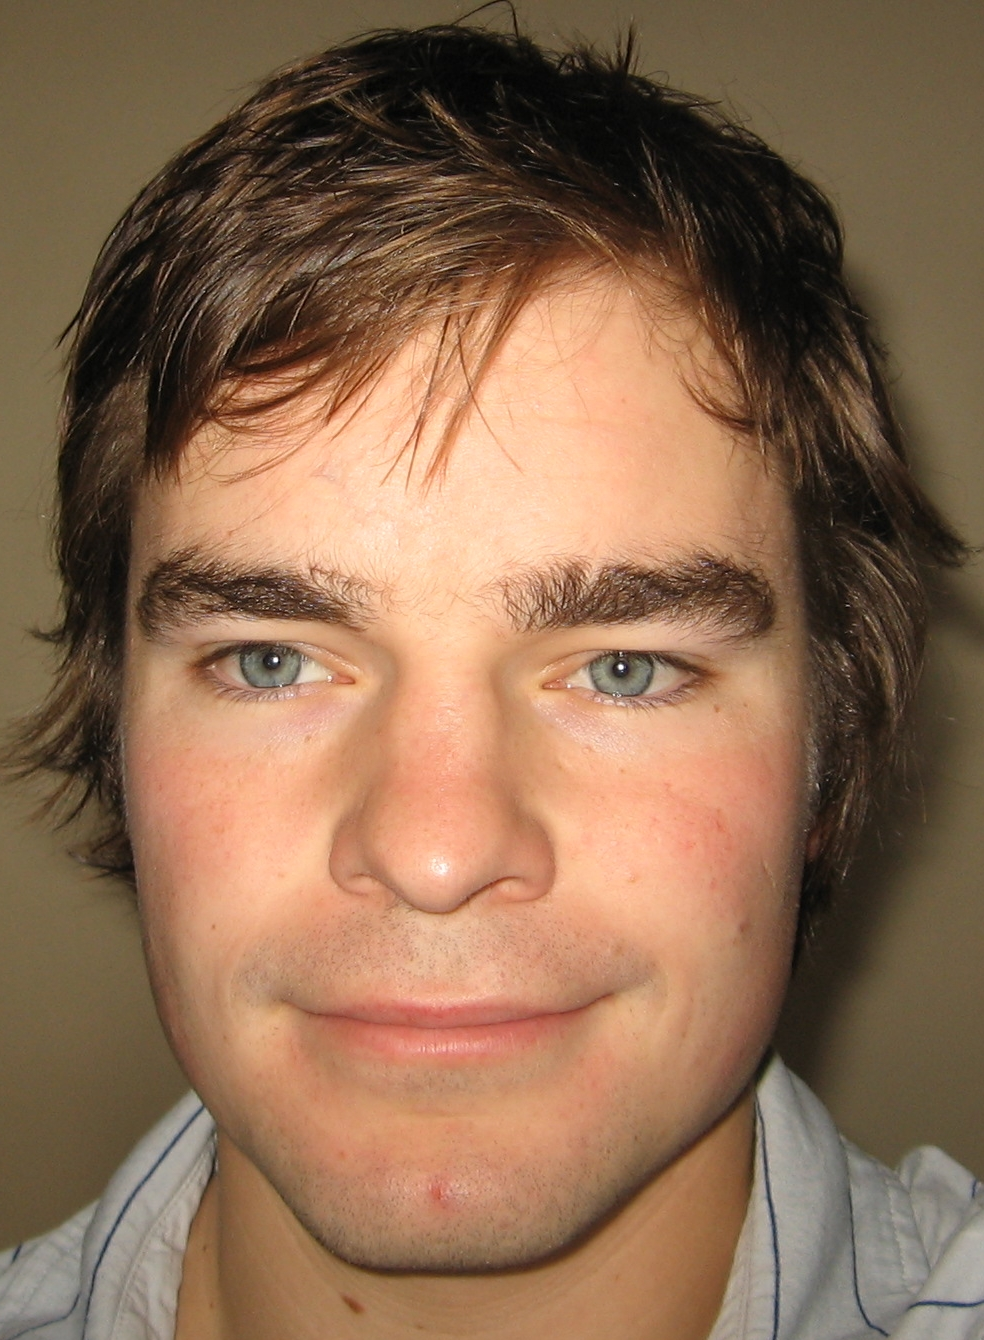
\includegraphics[width=1.2cm]{figures/tom} &
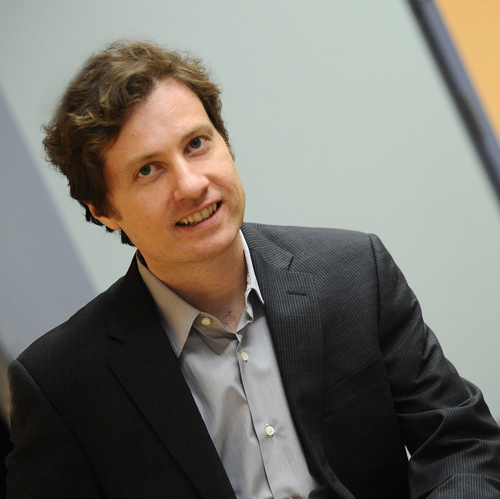
\includegraphics[width=1.5cm]{figures/collins} &
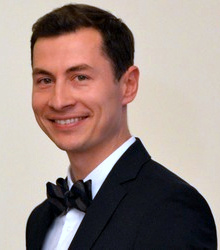
\includegraphics[width=1.4cm]{figures/petrov} \\
\footnotesize Tom~Kwiatkowski & \footnotesize Michael~Collins & \footnotesize Slav~Petrov \\
\end{tabular}
}
\end{center}
\end{frame}

\section{Introduction}

\begin{frame}
\frametitle{Syntax helps Semantics}
\centering
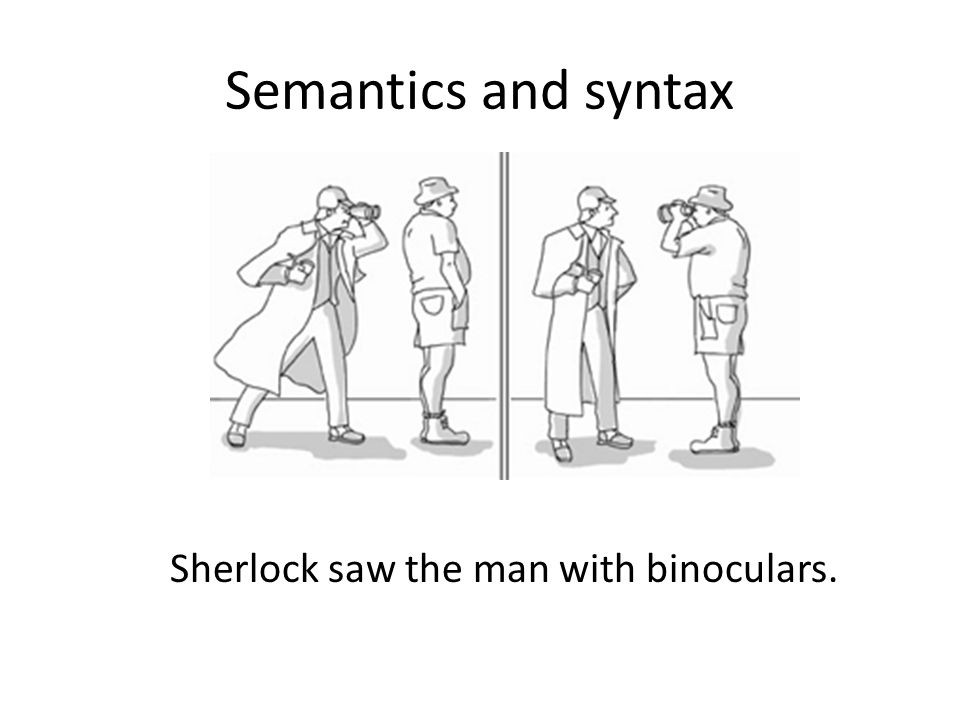
\includegraphics[trim=15em 18em 14em 12em,clip=true,scale=0.5]{figures/prep-ambiguity}

\vspace{2em}
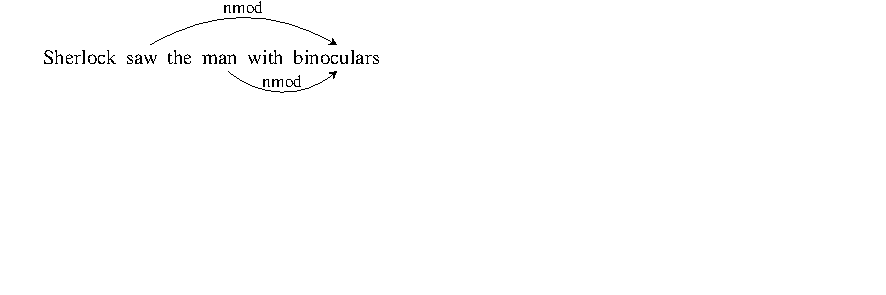
\includegraphics[trim=1em 9em 21em 0em,clip=true,scale=1.2]{figures/pp-ambiguity}
\end{frame}

\begin{frame}
\frametitle{Syntax helps Semantics}
\begin{center}
\only<1>{\vspace{-1em} 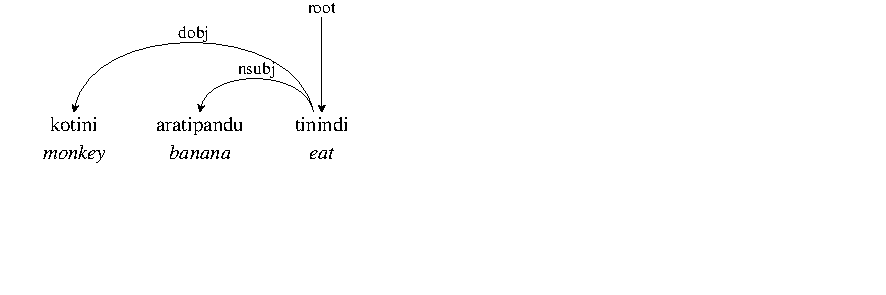
\includegraphics[trim=1em 5em 24em 5.1em,clip=true,scale=1.3]{figures/telugu-dependency-example} \\}
  \only<2>{\vspace{5em}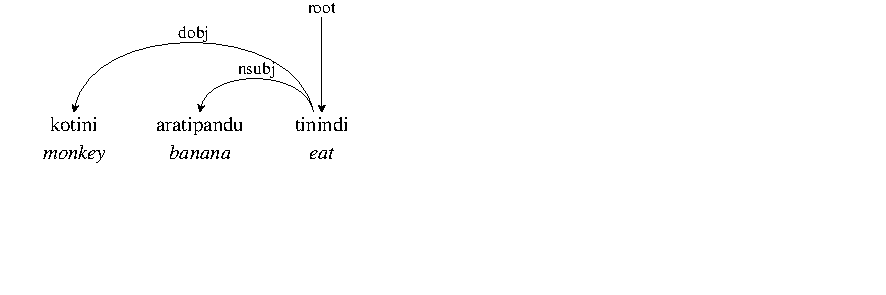
\includegraphics[trim=1em 5em 24em 5.1em,clip=true,scale=1.3]{figures/telugu-dependency-example} \\}
\only<3,4>{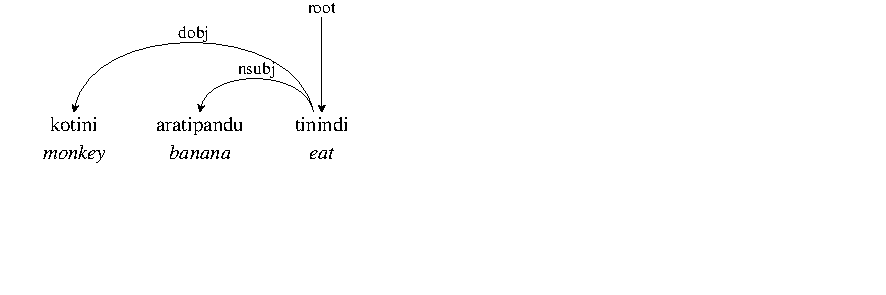
\includegraphics[trim=1em 5em 24em 0em,clip=true,scale=1.3]{figures/telugu-dependency-example} \\}
\only<2,3>{
\includegraphics[scale=0.45]{figures/monkey-eat-banana}}
\only<4>{
\includegraphics[scale=0.26]{figures/banana-eat-monkey}}
\end{center}
\end{frame}

\begin{frame}
\frametitle{Universal Dependencies}
%\large Homogeneous syntactic representation across languages
\begin{center}
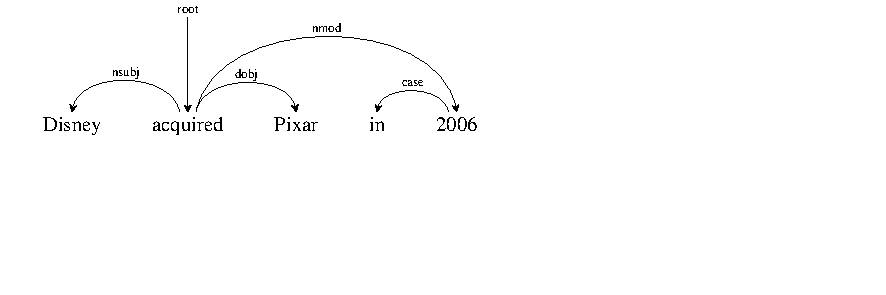
\includegraphics[trim=0em 5em 15em 0em,clip=true,scale=1.2
]{figures/dependency-word-order-english}

\only<1>{\vspace{4.8em}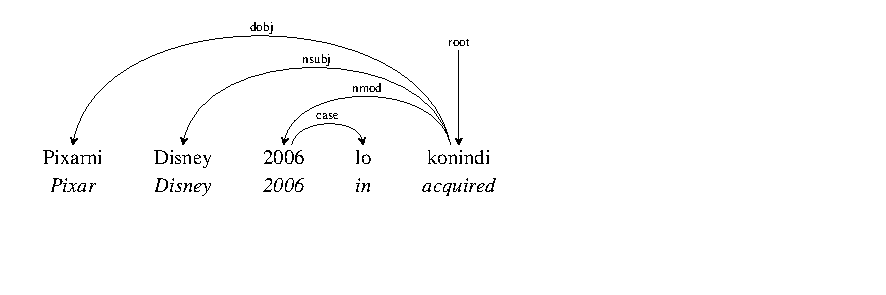
\includegraphics[trim=0em 3.5em 14em 6.5em,clip=true,scale=1.2
  ]{figures/dependency-word-order-telugu}}
\only<2>{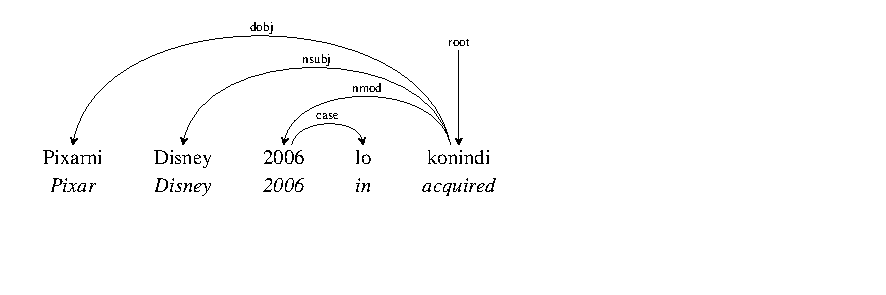
\includegraphics[trim=0em 3.5em 14em 0.5em,clip=true,scale=1.2
  ]{figures/dependency-word-order-telugu}
  \vspace{-0.5em}}
\end{center}
\end{frame} 

\begin{frame}[noframenumbering]
\frametitle{Universal Dependencies}
\large
Homogeneous syntactic representation across languages

\vspace{2em}
Treebanks in 40 languages

\vspace{2em}
40 dependency labels

\end{frame} 

\begin{frame}
\frametitle{Dependency Tree to Semantics}
\centering

\vspace{1em}

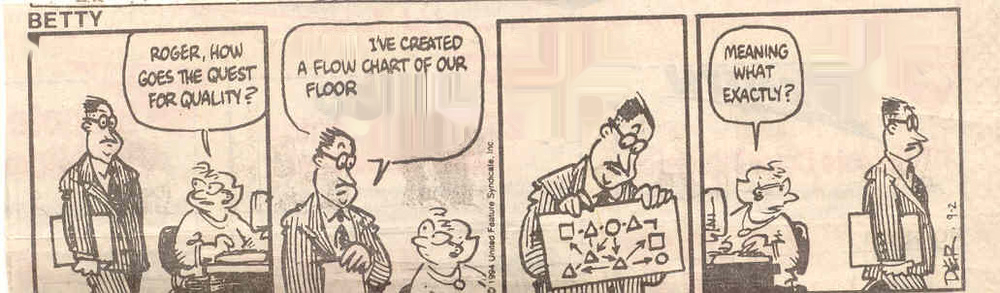
\includegraphics[trim=26em 0em 3.8em 2em,clip=true,scale=0.4]{figures/syntax-to-semantics-cartoon}

\vspace{2em}

\Large
  Dependencies \alert{lack} a formal theory of semantics
\end{frame}

\begin{frame}
 \frametitle{This Talk}
 \Large \centering
 
 A Compositional Typed Semantic Interface \\
 for Dependencies
\end{frame}

\begin{frame}
\frametitle{Dependency Tree to Semantics}
\large
\only<1>{
  \hlight{Principle of Compositionality:} the semantics of a complex expression is determined by the semantics of its constituent expressions and the rules used to combine them}
\only<2>{
  \hlight{Principle of Compositionality:} the semantics of a \alert{complex expression} is determined by the semantics of its constituent expressions and the rules used to combine them}
\only<3>{
  \hlight{Principle of Compositionality:} the semantics of a \alert{complex expression} is determined by the semantics of its {\color{darkgreen}
 constituent expressions} and the rules used to combine them}
\only<4>{
  \hlight{Principle of Compositionality:} the semantics of a \alert{complex expression} is determined by the semantics of its {\color{darkgreen}
    constituent expressions} and the {\color{purple} rules} used to combine them}
  
  \visible<2->{
  \vspace{2em}
  \alert{Complex expression} is the dependency tree}
  
\visible<3->{
  \vspace{2em}
  {\color{darkgreen} Constituent expressions} are subtrees}
  

\visible<4->{
  \vspace{2em}
  {\color{purple} Rules} are the dependency labels
}
\end{frame}

\begin{frame}
\frametitle{Existing Syntax-Semantics interfaces}
\large
CCG {\scriptsize [Steedman, 2000; Bos et al., 2004]}
  
\vspace{2em}
  HPSG {\scriptsize [Copestake et al., 2001]}
  
\vspace{2em}
LFG {\scriptsize [Dalrymple et al., 1995]}
  
\vspace{2em}
TAG {\scriptsize [Joshi et al., 1995]}
\end{frame}


\begin{frame}
\frametitle{CCG}
\centering
\only<1>{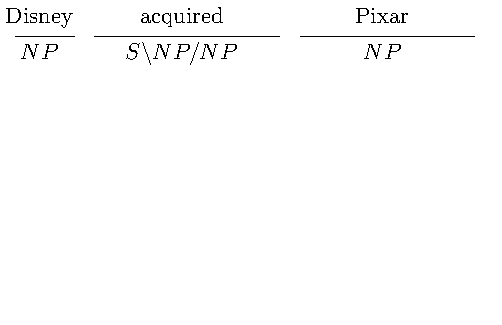
\includegraphics[trim=0em 1em 1em 0em,clip=true,scale=1.2]{figures/ccg-transitive1}} 
\only<2,4>{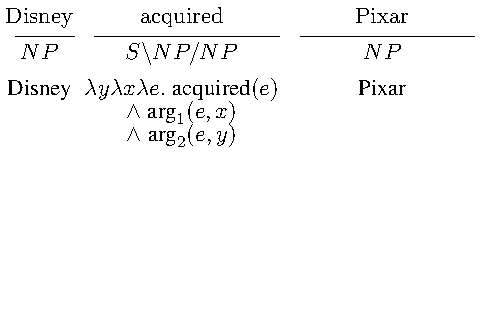
\includegraphics[trim=0em 1em 1em 0em,clip=true,scale=1.2]{figures/ccg-transitive2}}
\only<3>{
  \vspace{1em}
  \begin{block}{\centering Lambda Calculus}
    \centering $(\lambda x.M)N = M[x := N]$ 
\end{block}

\begin{align*}
sum(2,3) & =  (\lambda x \lambda  y \lspace (+\;\; x \;\;\; y))(2)(3) \\
 &  = (\lambda y \lspace (+\;\; 2 \;\;\; y))(3) \\
\pause
  & = (+\;\; 2 \;\;\; 3) \\
  & = 5 \\
  \\
\type{sum} & =   int \rightarrow int \rightarrow int \\
sum(4,sum(2,3)) & = 9 \\
\end{align*}
}
\only<5>{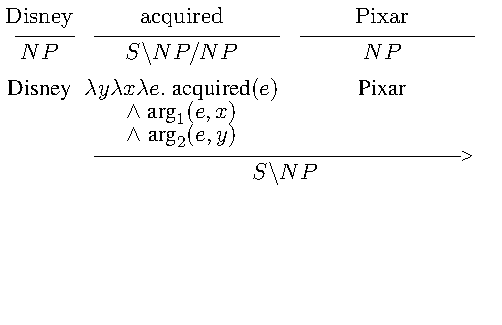
\includegraphics[trim=0em 1em 1em 0em,clip=true,scale=1.2]{figures/ccg-transitive3}}
\only<6>{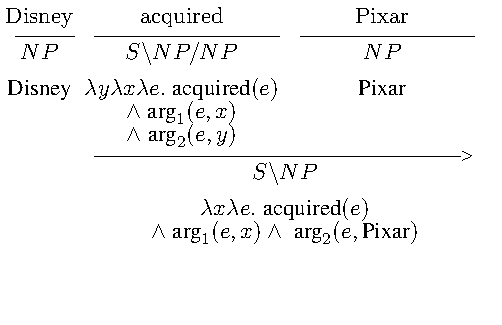
\includegraphics[trim=0em 1em 1em 0em,clip=true,scale=1.2]{figures/ccg-transitive4}}
\only<7,8>{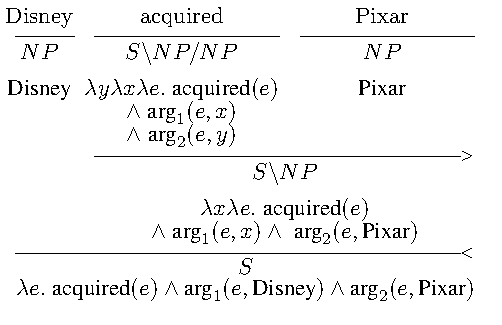
\includegraphics[trim=0em 1em 1em 0em,clip=true,scale=1.2]{figures/ccg-transitive}}

\only<8>{
\vspace{1em}
Typing and Combinator Rules allow \\Synchronous Syntax-Semantics interface
\vspace{-3em}}
\end{frame}

\begin{frame}
\frametitle{Why from dependencies?}
\large

Easy to annotate

\vspace{2em}
Treebanks in many languages

\vspace{2em}
Very accurate parsers\\
{\footnotesize [Andor et al., 2016, Dyer et al., 2015, Chen \& Manning, 2014]}


\vspace{2em}
Friendly to read
\end{frame}

\begin{frame}
\frametitle{Outline}
\large 
DepLambda: Dependencies to Logical Forms
 
\vspace{2em}
Freebase Semantic Parsing using DepLambda

\vspace{2em}
Results on English, German, and Spanish

\blfootnote{
\color{blue}
 $\bullet$ Reddy, T\"ackstr\"om, Collins, Kwiatkowski, Das, Steedman, Lapata (TACL 2016) \\
 \hspace{1.5em} $\bullet$ Reddy, Lapata, Steedman (TACL 2014)
}
\end{frame}

\begin{frame}
\Large
\centering
\vspace{1.5em}
DepLambda: \\
 Dependencies to Logical Forms
\end{frame}

\begin{frame}
\frametitle{Dependencies to Logical Forms}
\vspace{-1em}
\begin{center}
\only<1>{\vspace{-5em}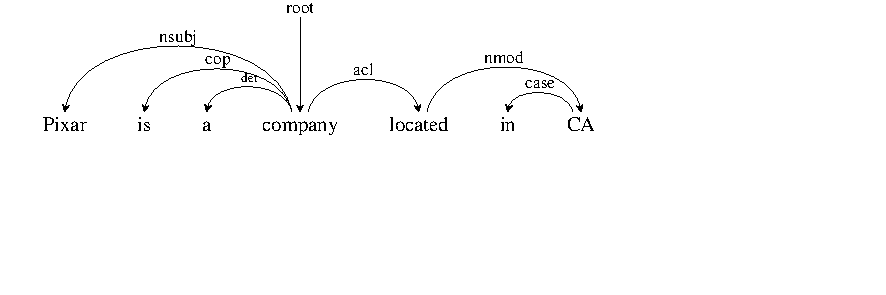
\includegraphics[trim=2em 5em 12em 0em,clip=true,scale=1.0]{figures/dependency-reduced-relative-ud}}
\only<2>{\vspace{2em}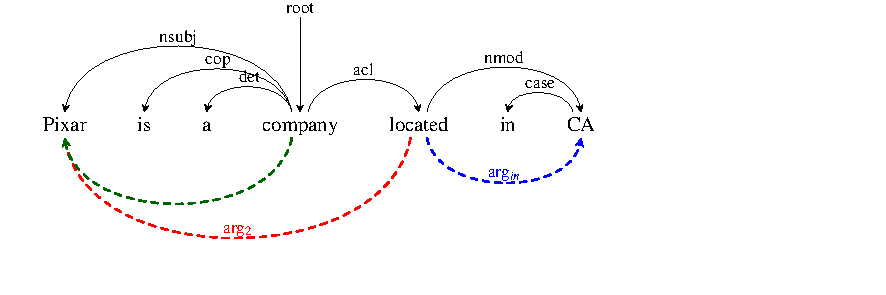
\includegraphics[trim=2em 2em 12em 0em,clip=true,scale=1.0]{figures/dependency-reduced-relative-ud-parg}}
\only<3,4>{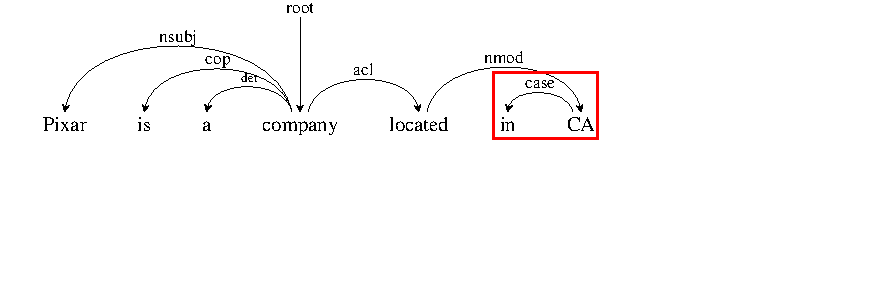
\includegraphics[trim=2em 5em 12em 0em,clip=true,scale=1.0]{figures/dependency-reduced-relative-ud-box1}}
\only<5,6>{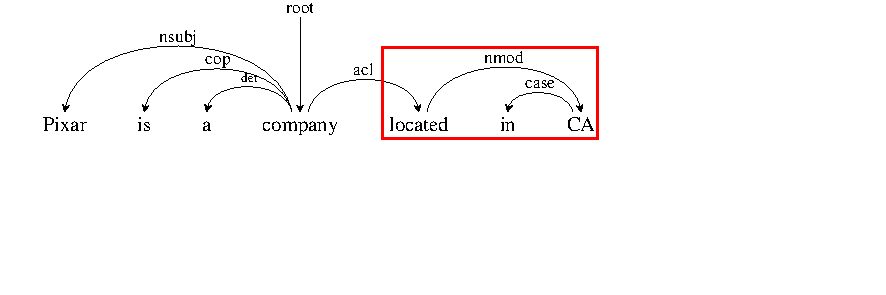
\includegraphics[trim=2em 5em 12em 0em,clip=true,scale=1.0]{figures/dependency-reduced-relative-ud-box2}}
\only<7>{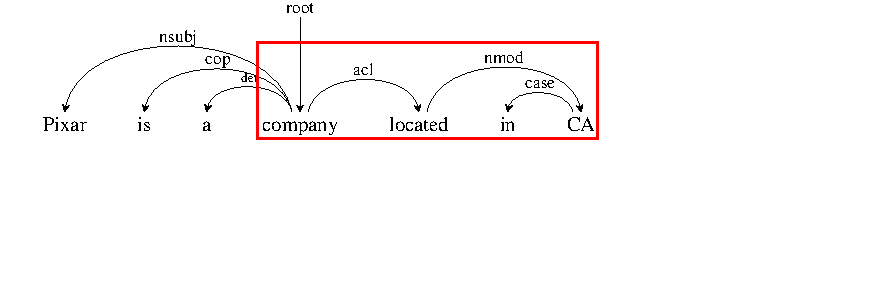
\includegraphics[trim=2em 5em 12em 0em,clip=true,scale=1.0]{figures/dependency-reduced-relative-ud-box3}}
\only<8->{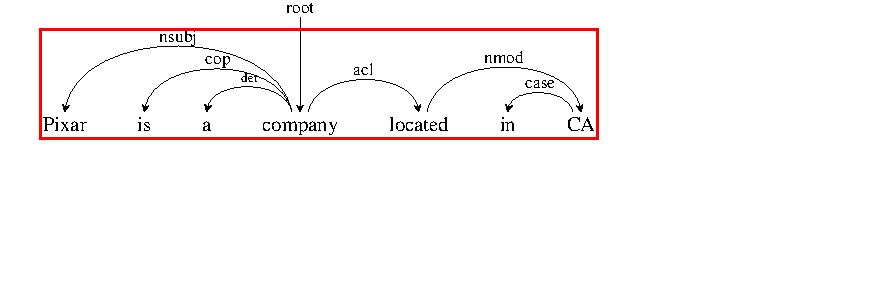
\includegraphics[trim=1.5em 5em 12em 0em,clip=true,scale=1.0]{figures/dependency-reduced-relative-ud-box4}}
 
\only<3>{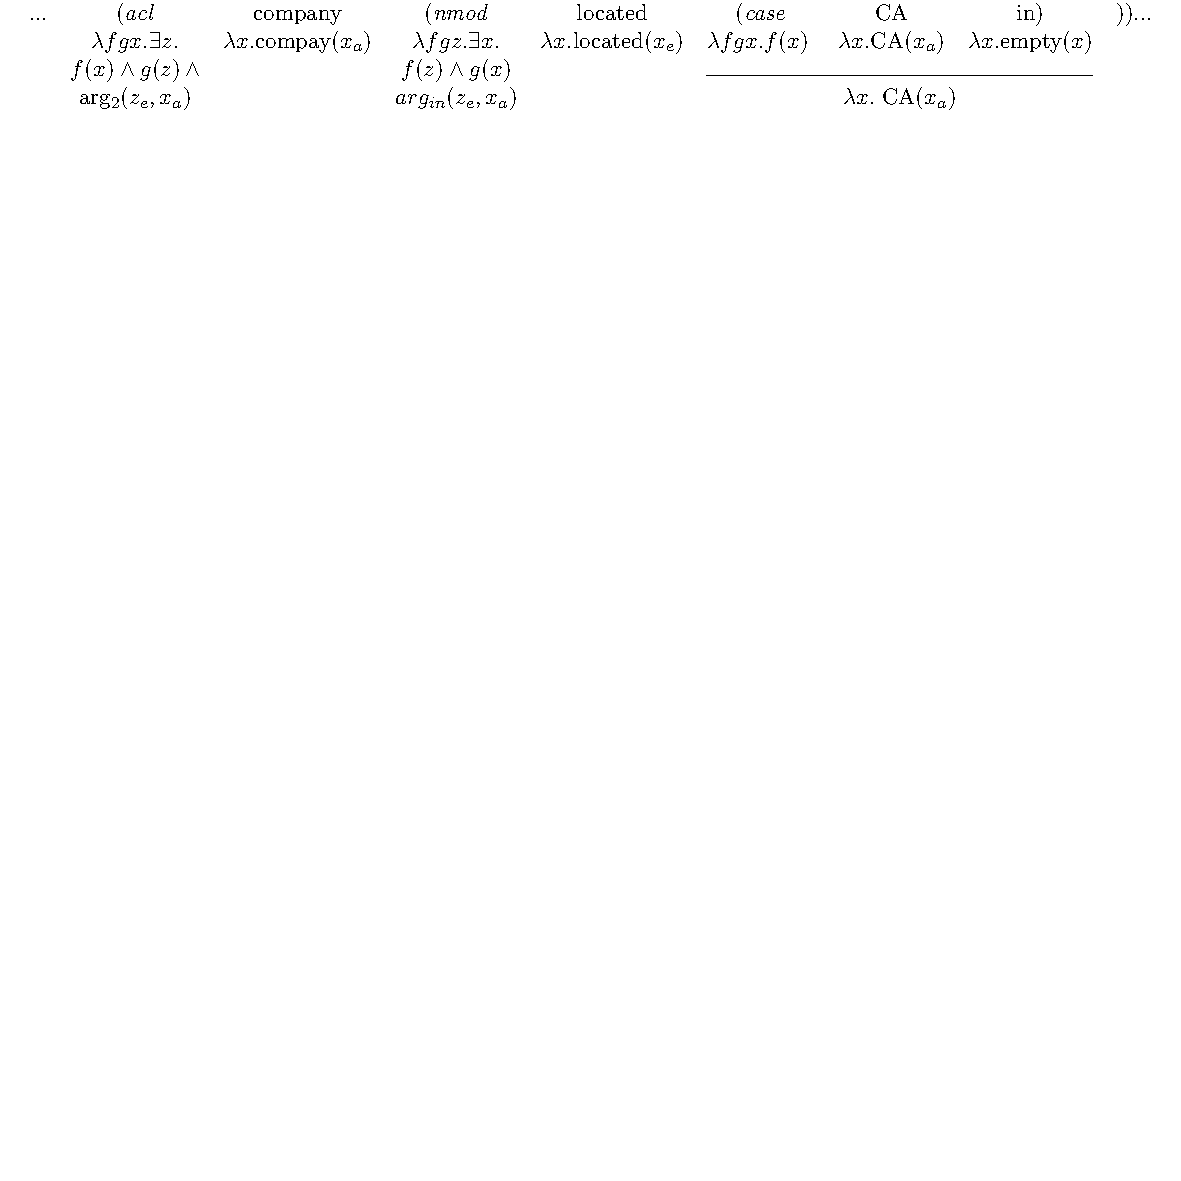
\includegraphics[trim=29.5em 51.5em 4.5em 0em,clip=true,scale=0.9]{figures/dependency-reduced-relative-derivation-ud}\vspace{6.5em}}
\only<4>{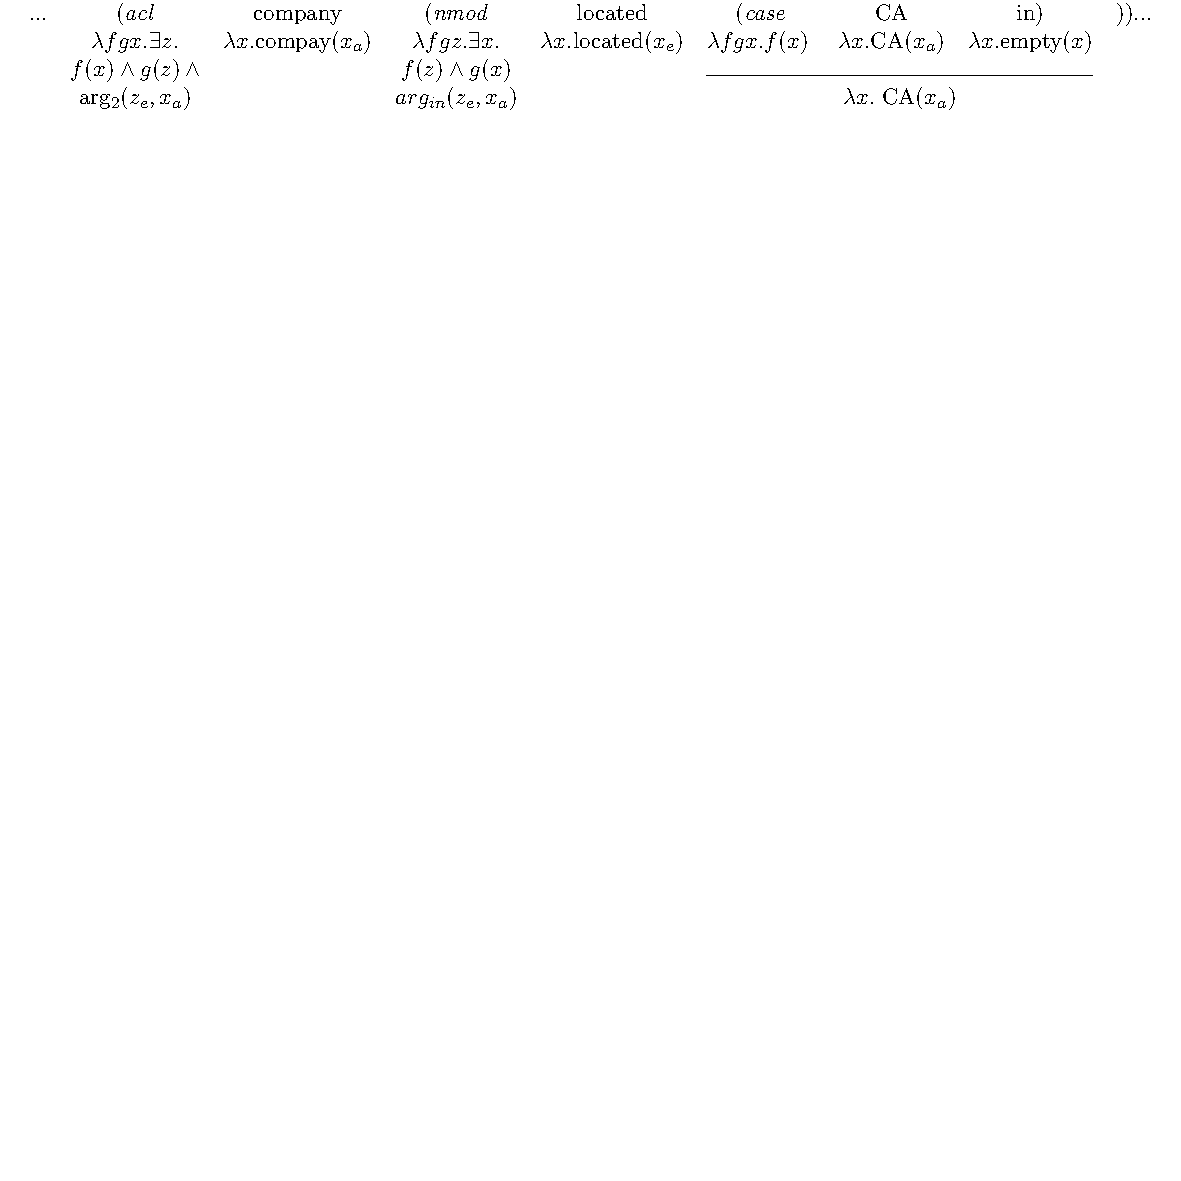
\includegraphics[trim=29.5em 51.5em 4.5em 0em,clip=true,scale=0.9]{figures/dependency-reduced-relative-derivation-ud}\\
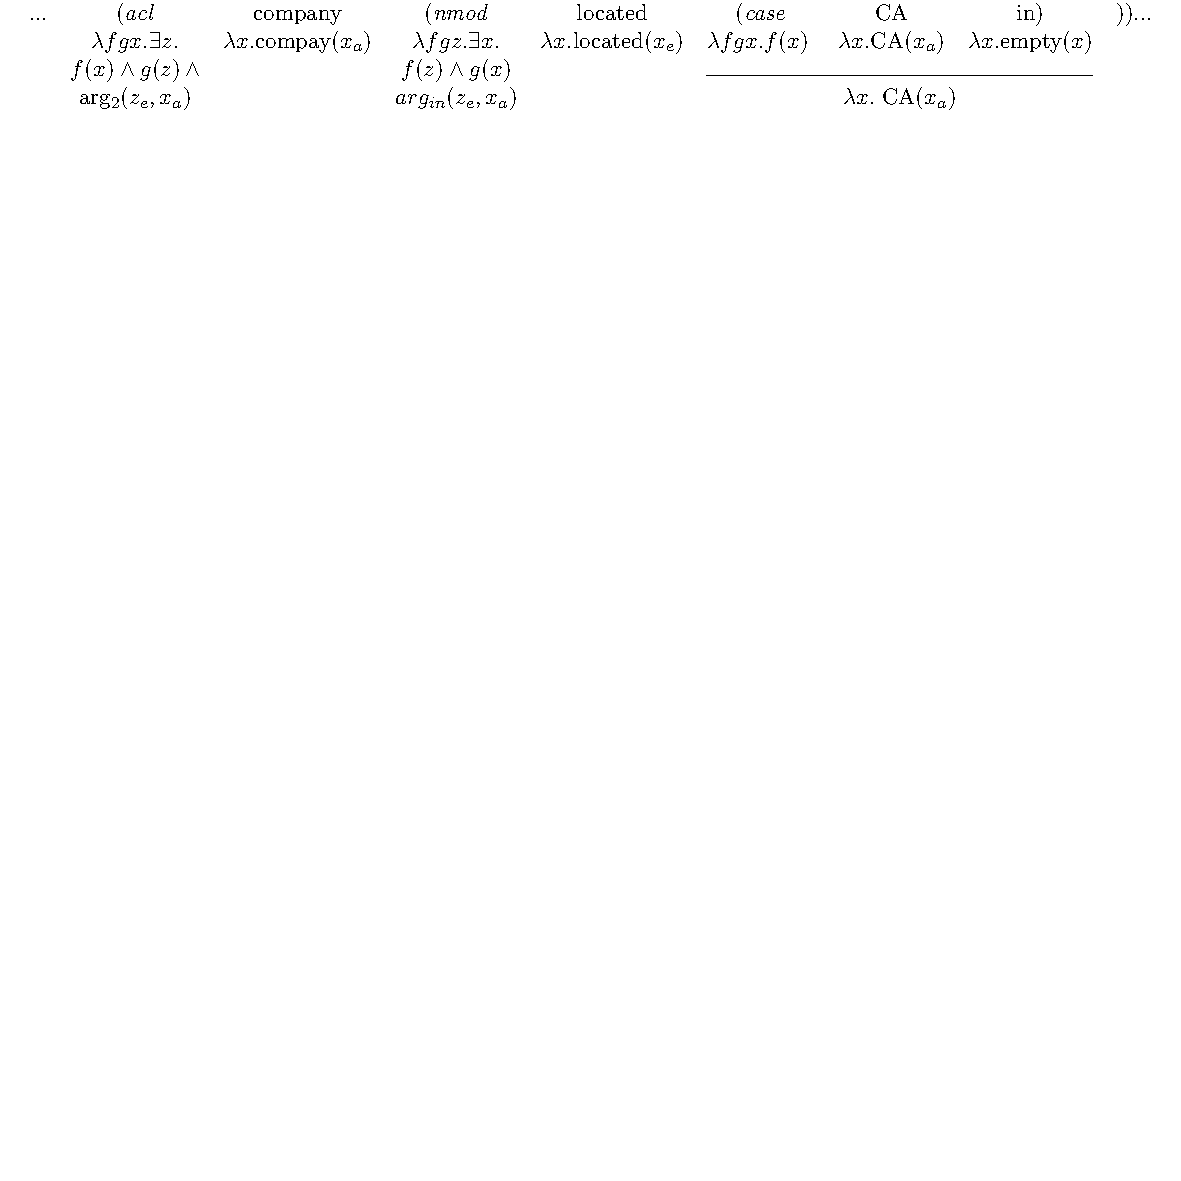
\includegraphics[trim=30.6em 45em 6em 3em,clip=true,scale=0.9]{figures/dependency-reduced-relative-derivation-ud}\vspace{2em}}
\only<5>{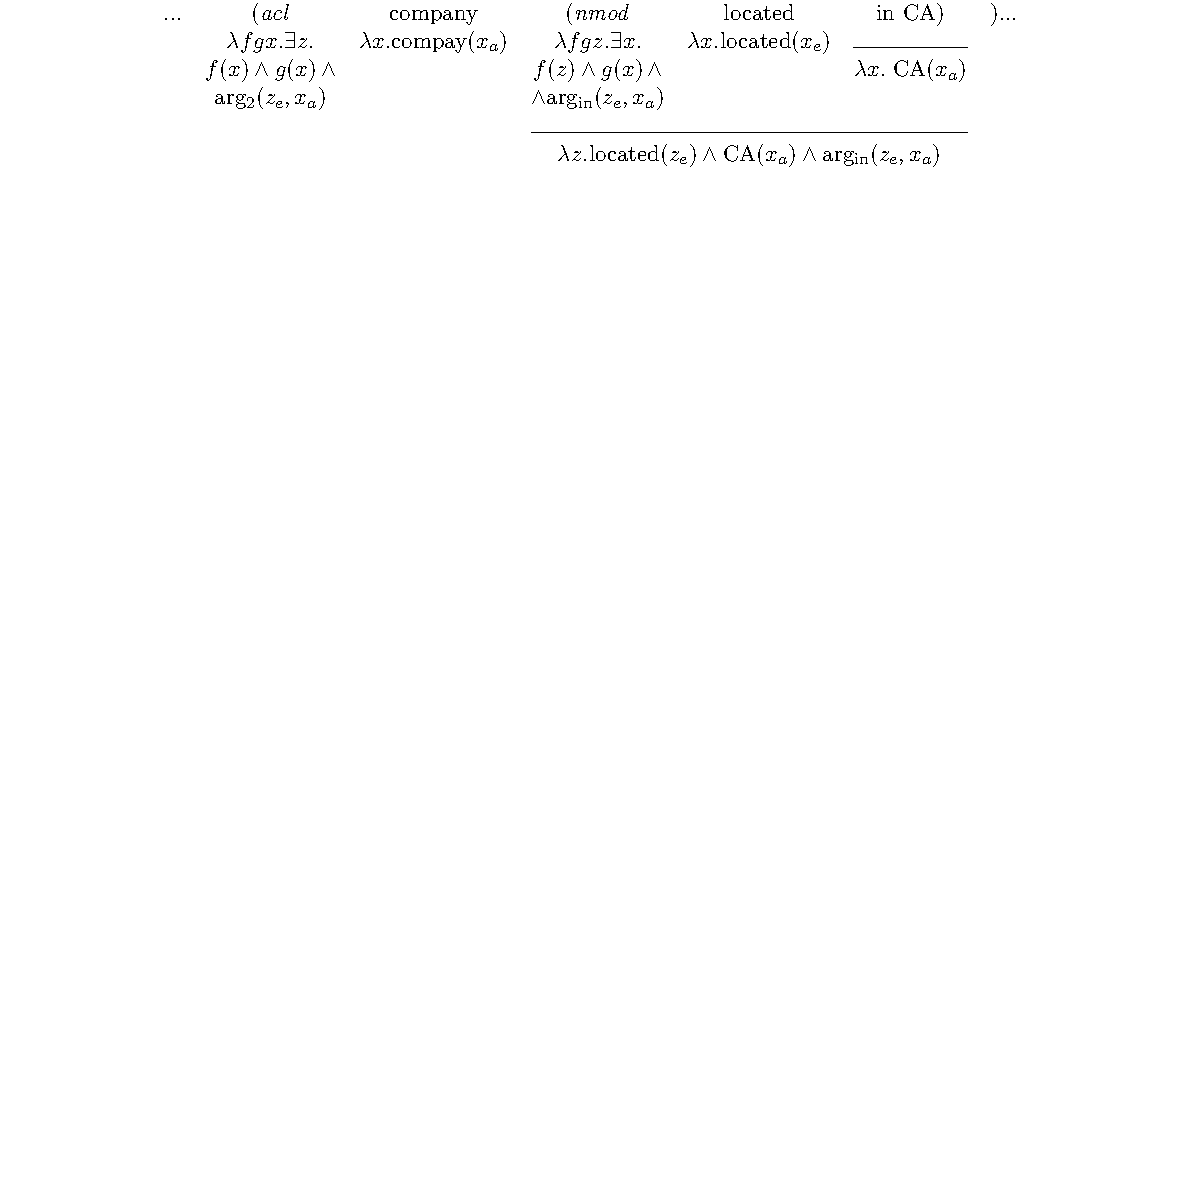
\includegraphics[trim=22em 51.5em 9em 0em,clip=true,scale=0.9]{figures/dependency-reduced-relative-derivation1-ud}\vspace{6.5em}} 
\only<6>{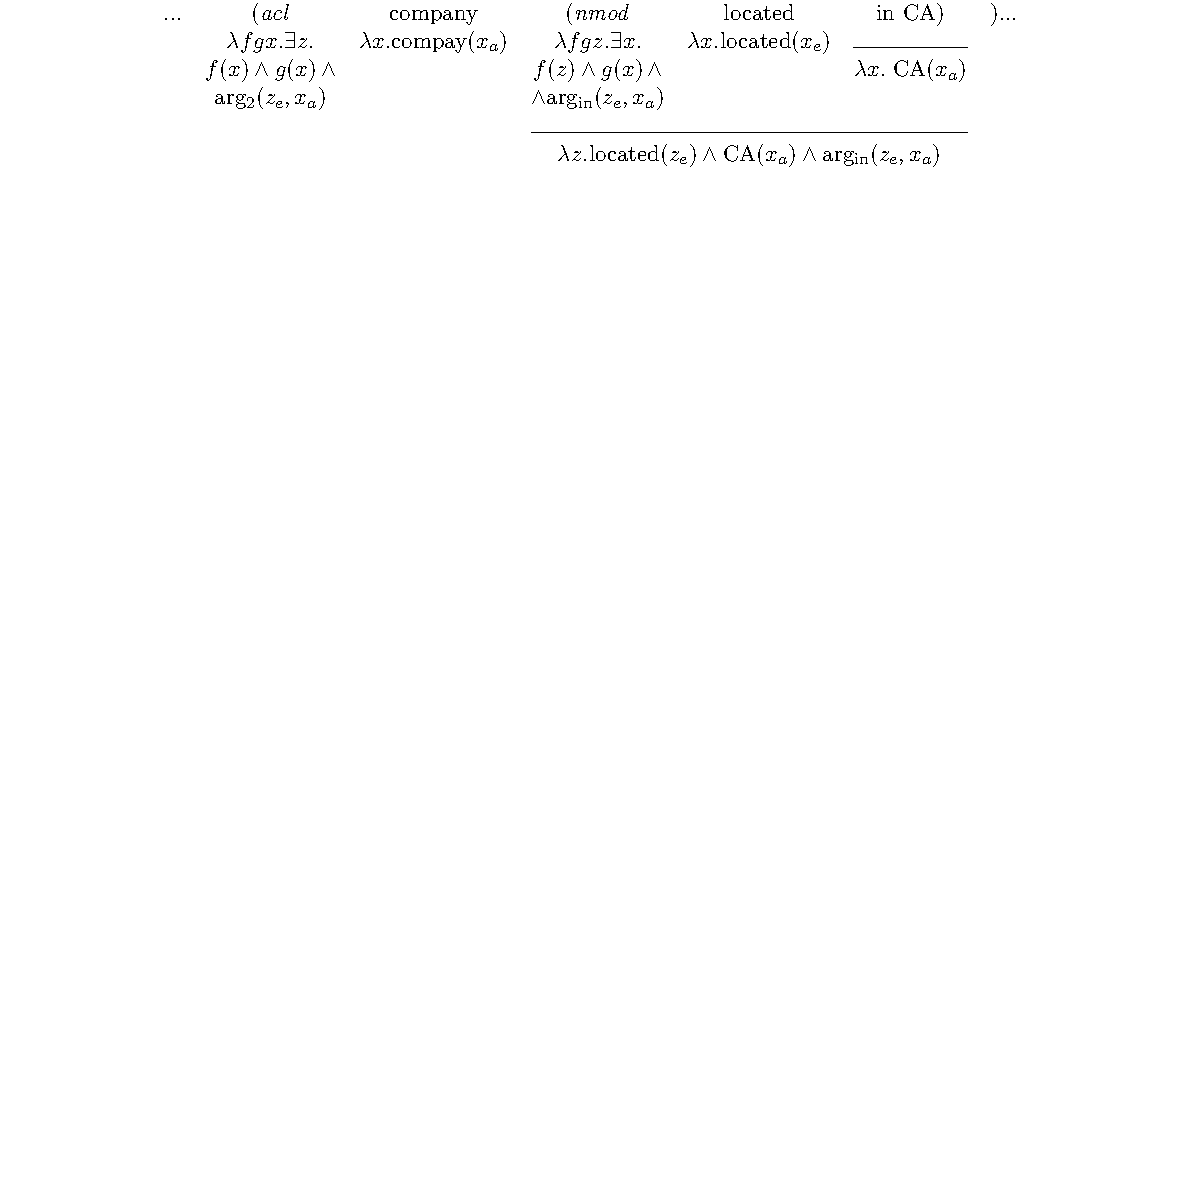
\includegraphics[trim=22em 51.5em 9em 0em,clip=true,scale=0.9]{figures/dependency-reduced-relative-derivation1-ud}\\
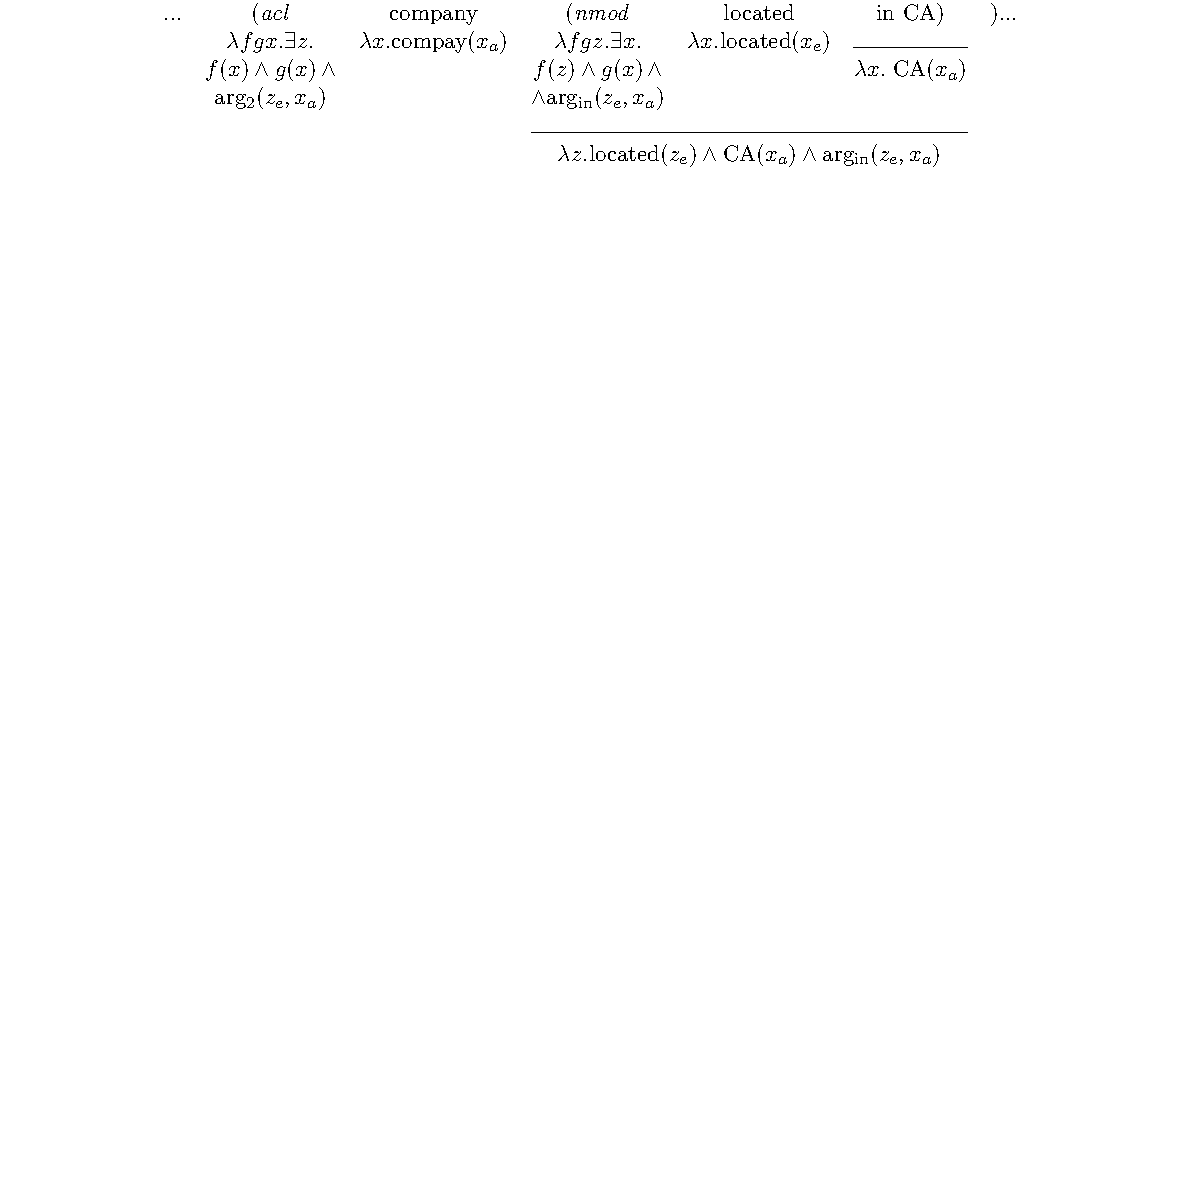
\includegraphics[trim=23em 45em 9em 5em,clip=true,scale=0.9]{figures/dependency-reduced-relative-derivation1-ud}\vspace{4em}}
\only<7>{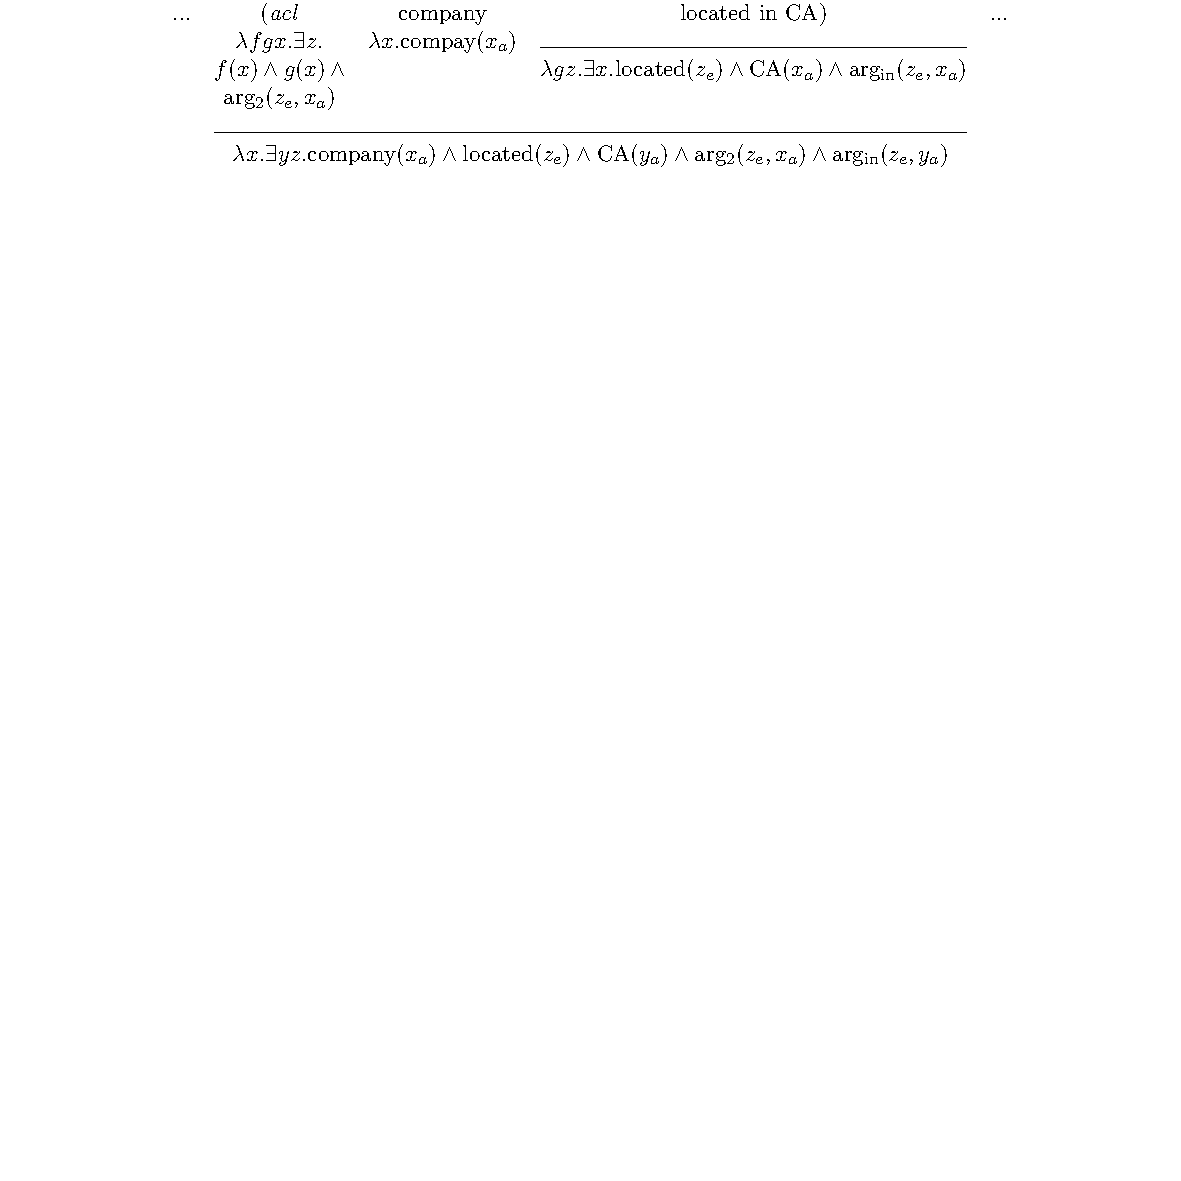
\includegraphics[trim=9em 51.3em 9em 0em,clip=true,scale=0.9]{figures/dependency-reduced-relative-derivation2-ud}\\
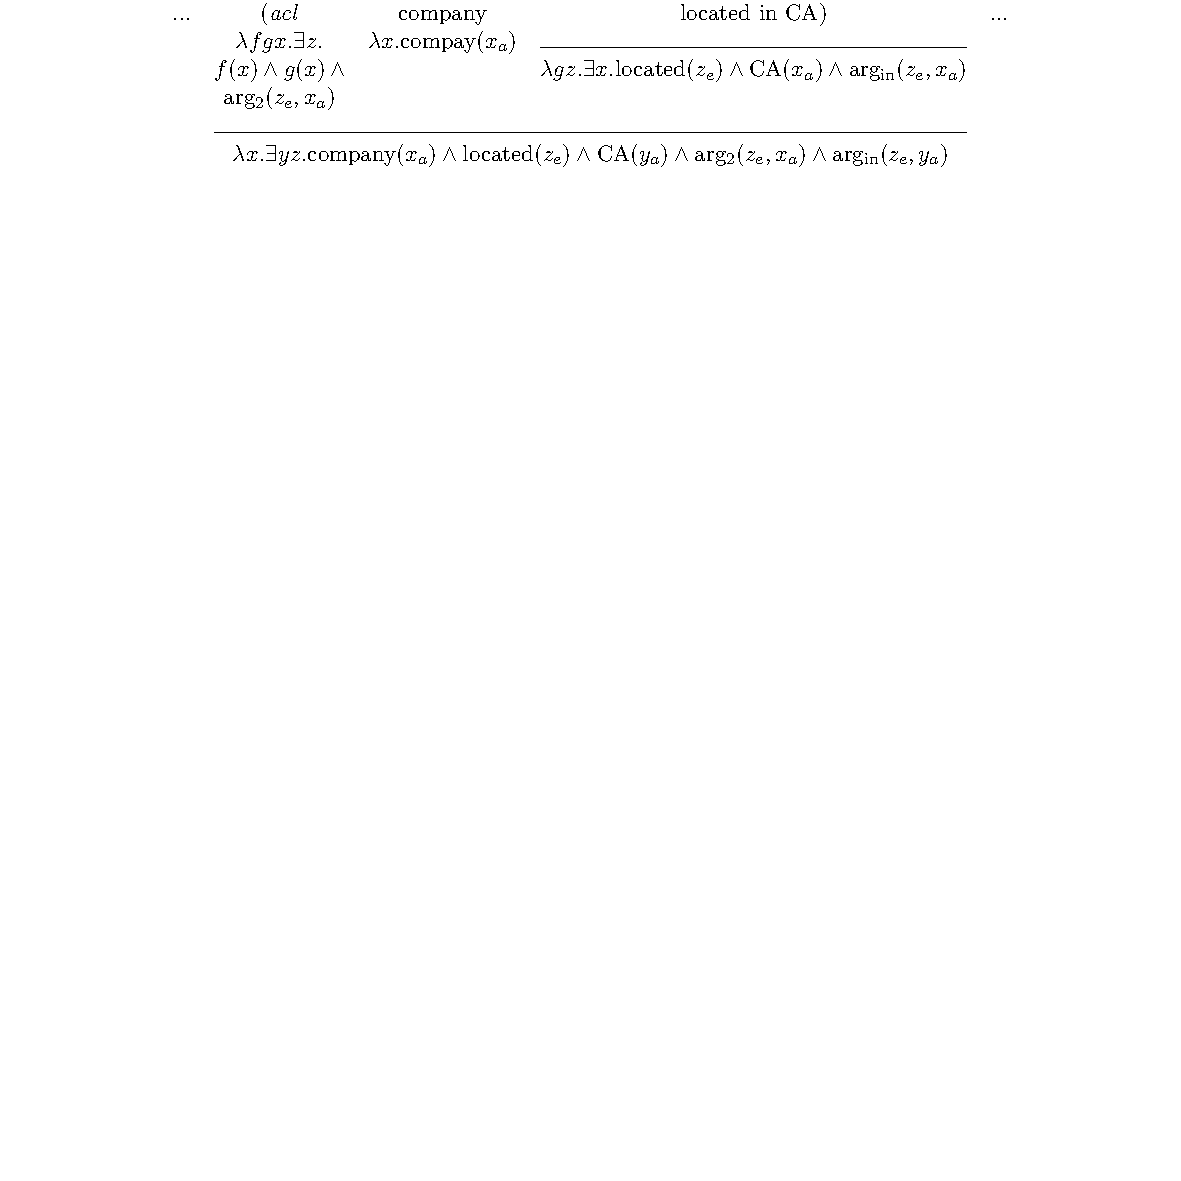
\includegraphics[trim=9em 45em 9em 5.5em,clip=true,scale=0.9]{figures/dependency-reduced-relative-derivation2-ud}\vspace{4em}} 

\only<2>{\vspace{2cm}$\lambda x. \exists yz \lspace \mathrm{located}(z_e) \wedge  \mathrm{Pixar}(x_a) \wedge \mathrm{CA}(y_a) \wedge$ \\ $\mathrm{\color{darkgreen}company(x_a)} \wedge \mathrm{\color{red}arg_2}(z_e, x_a) \wedge \mathrm{\color{blue} arg_{in}}(z_e, y_a)$}
\only<8>{\vspace{2cm}$\lambda x. \exists yz \lspace \mathrm{located}(z_e) \wedge  \mathrm{Pixar}(x_a) \wedge \mathrm{CA}(y_a) \wedge$ \\ $\mathrm{company(x_a)} \wedge \mathrm{arg_2}(z_e, x_a) \wedge \mathrm{arg_{in}}(z_e, y_a)$}
\end{center} 
\end{frame}

\begin{frame}
\frametitle{Dependencies to Logical Forms}
\begin{center}
\vspace{1em}
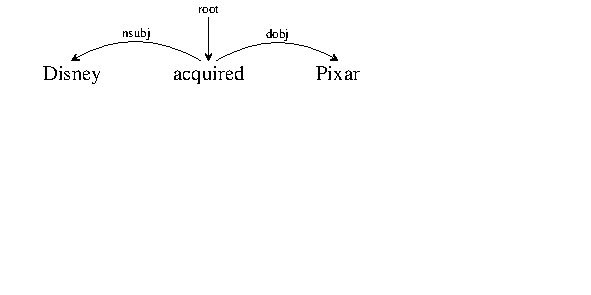
\includegraphics[trim=2em 9.4em 10em 0em,clip=true,scale=1.3]{figures/pixar}

\vspace{4cm}

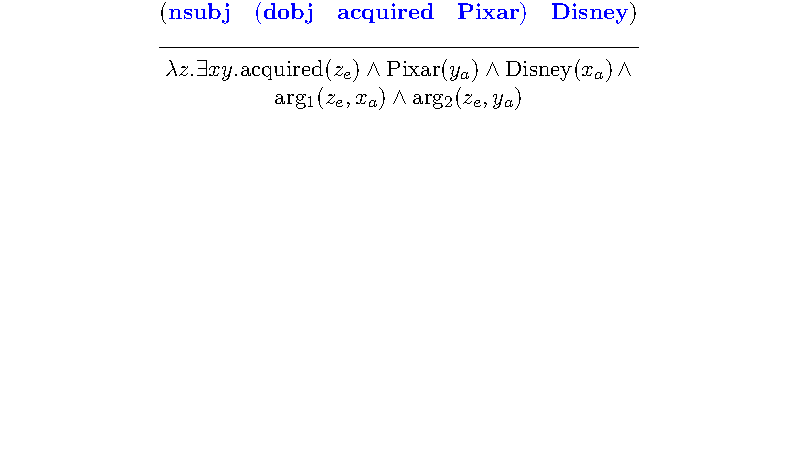
\includegraphics[trim=7em 10em 7em 2.5em,clip=true,scale=1.1]{figures/dependency-transitive-derivation_full}
\vspace{-2cm}
\end{center}
\end{frame}

\subsection{Single Type System}
\begin{frame}
\frametitle{Dependencies to Logical Forms}
\framesubtitle{Our Approach}
\begin{center}
\vspace{-5em}
% TODO: remove types on dependency labels.
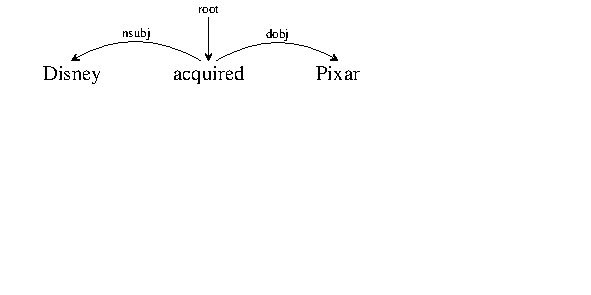
\includegraphics[trim=2em 9.4em 10em 0em,clip=true,scale=1.3]{figures/pixar}

\vspace{2cm}
\begin{block}{}
\centering
Let dependency labels drive the composition
\end{block}
\end{center}
\end{frame}

\begin{frame}[noframenumbering]
\frametitle{Dependencies to Logical Forms}
\framesubtitle{Our Approach}
\vspace{-2.5em}
\centering

\only<1>{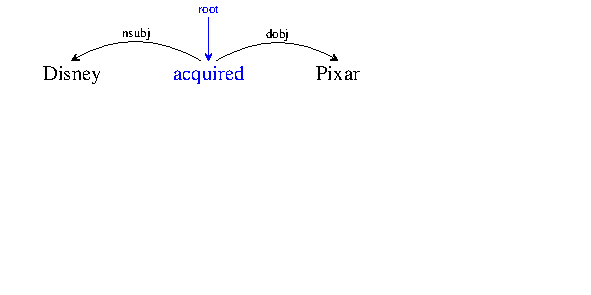
\includegraphics[trim=2em 9.4em 10em 0em,clip=true,scale=1.3]{figures/pixar_root}}
\only<2->{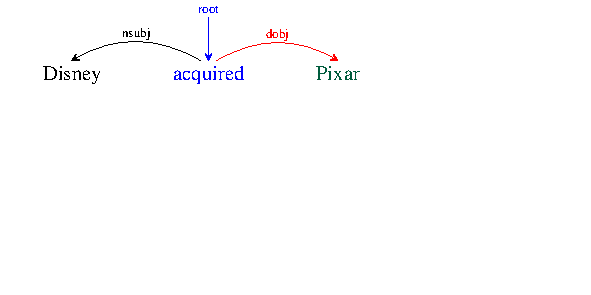
\includegraphics[trim=2em 9.4em 10em 0em,clip=true,scale=1.3]{figures/pixar_dobj}}

\tikz[remember picture] \node[coordinate] (n1) {};\\
\vspace{2cm}
\tikz[remember picture] \node[coordinate] (n2) {};

\begin{tikzpicture}[remember picture,overlay]   %% use here too
  \draw [->,>=stealth,shorten >=1pt,blue!20!white,line width=10pt] (n1) -- node[xshift=6em,black] {\footnotesize $\ldots >$ dobj $> \dots >$  nsubj $> \ldots$ } (n2);
  \draw [->,>=stealth,blue!20!white,sloped,line width=10pt] (n1) -- node[black] {\footnotesize obliqueness} (n2);
\end{tikzpicture}

\visible<2->{({\color{red} dobj} {\color{blue} acquired} {\color{blue!40!green!60!black} Pixar})}
\end{frame}

\begin{frame}[noframenumbering]
\frametitle{Dependencies to Logical Forms}
\framesubtitle{Our Approach}
\vspace{-2.5em}
\centering

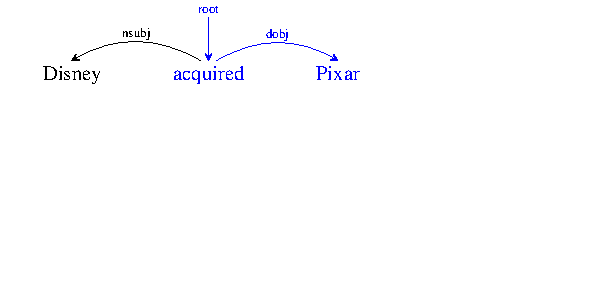
\includegraphics[trim=2em 9.4em 10em 0em,clip=true,scale=1.3]{figures/pixar_dobj_phrase}

\tikz[remember picture] \node[coordinate] (n1) {};\\
\vspace{2cm}
\tikz[remember picture] \node[coordinate] (n2) {};

\begin{tikzpicture}[remember picture,overlay]   %% use here too
  \draw [->,>=stealth,shorten >=1pt,blue!20!white,line width=10pt] (n1) -- node[xshift=6em,black] {\footnotesize $\ldots >$ dobj $> \dots >$  nsubj $> \ldots$ } (n2);
  \draw [->,>=stealth,blue!20!white,sloped,line width=10pt] (n1) -- node[black] {\footnotesize obliqueness} (n2);
\end{tikzpicture}

{\color{blue} (dobj acquired Pixar)}
\end{frame}

\begin{frame}[noframenumbering]
\frametitle{Dependencies to Logical Forms}
\framesubtitle{Our Approach}
\vspace{-2.5em}
\centering

\only<1>{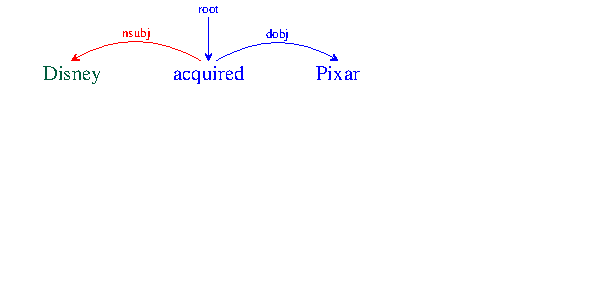
\includegraphics[trim=2em 9.4em 10em 0em,clip=true,scale=1.3]{figures/pixar_nsubj}}
\only<2->{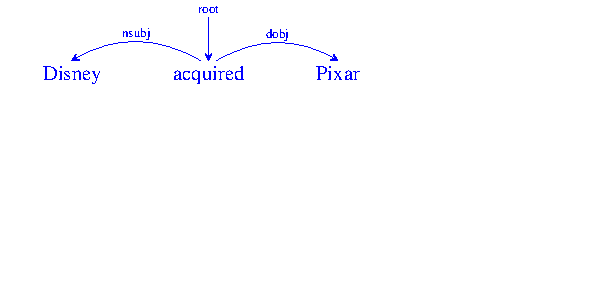
\includegraphics[trim=2em 9.4em 10em 0em,clip=true,scale=1.3]{figures/pixar_nsubj_phrase}}

\tikz[remember picture] \node[coordinate] (n1) {};\\
\vspace{2cm}
\tikz[remember picture] \node[coordinate] (n2) {};

\begin{tikzpicture}[remember picture,overlay]   %% use here too
  \draw [->,>=stealth,shorten >=1pt,blue!20!white,line width=10pt] (n1) -- node[xshift=6em,black] {\footnotesize $\ldots >$ dobj $> \dots >$  nsubj $> \ldots$ } (n2);
  \draw [->,>=stealth,blue!20!white,sloped,line width=10pt] (n1) -- node[black] {\footnotesize obliqueness} (n2);
\end{tikzpicture}

\only<1>{({\color{red} nsubj} {\color{blue} (dobj acquired Pixar)} {\color{blue!40!green!60!black} Disney})}
\only<2->{\color{blue}(nsubj (dobj acquired Pixar) Disney)}
\end{frame}

\begin{frame}[noframenumbering]
\frametitle{Dependencies to Logical Forms}
\framesubtitle{Our Approach}
\begin{center}
%\vspace{-1em}
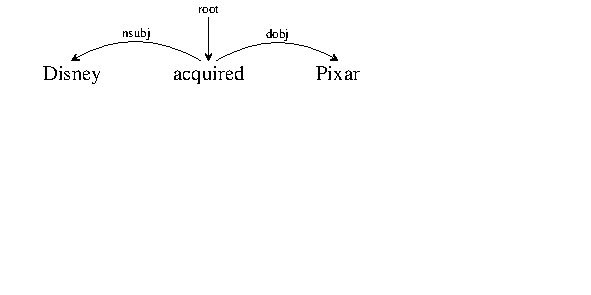
\includegraphics[trim=2em 9.4em 10em 0em,clip=true,scale=1.3]{figures/pixar}

\vspace{3em}
(nsubj (dobj acquired Pixar) Disney)
\vspace{3em}

\visible<1->{
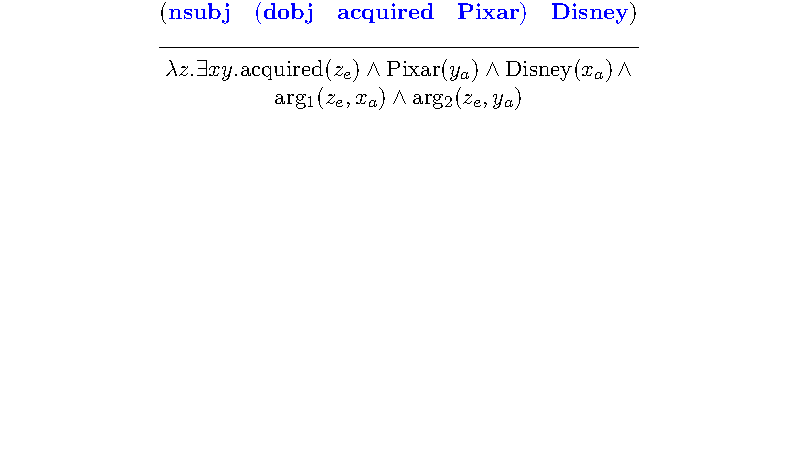
\includegraphics[trim=7em 0em 7em 2.5em,clip=true,scale=1.1]{figures/dependency-transitive-derivation_full}
\vspace{-1.5cm}}
\end{center}
\end{frame}

\begin{frame}
\frametitle{Dependencies to Logical Forms}
\framesubtitle{Lambda Calculus}
\vspace{-3.3em}
\begin{center}
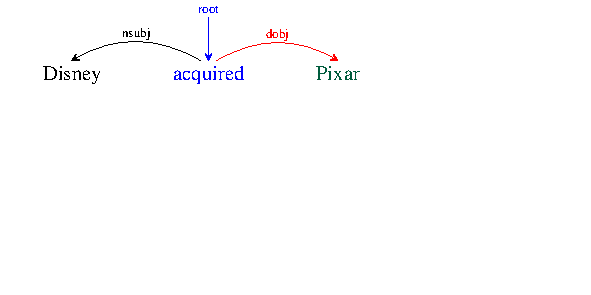
\includegraphics[trim=2em 9.4em 10em 0em,clip=true,scale=1.3]{figures/pixar_dobj}

\end{center}

\vspace{1cm}

\begin{block}{Lambda Calculus Basic Types}
\begin{itemize}
  \item Individuals: $\itype$ (also denoted by $._a$)
  \item Events: $\etype$ (also denoted by $._e$)
  \item Truth values: $\btype$
\end{itemize}
\end{block}
\end{frame}

\begin{frame}[noframenumbering]
\frametitle{Dependencies to Logical Forms}
\framesubtitle{Lambda Calculus}
\vspace{-2.4em}
\begin{center}
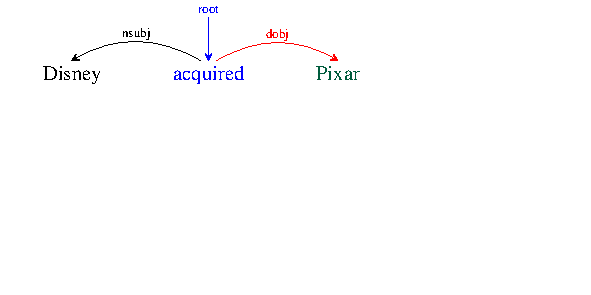
\includegraphics[trim=2em 9.4em 10em 0em,clip=true,scale=1.3]{figures/pixar_dobj}

\end{center}

\vspace{1cm}

\begin{block}{\centering Lambda Expression for words}
\vspace{-0.5cm}
\begin{align*}
  \hbox{\color{blue} acquired} & \Rightarrow  \lambda x \lspace \hbox{acquired}(x_e)  \\
  \hbox{\color{blue!40!green!60!black} Pixar} & \Rightarrow  \lambda x \lspace \hbox{Pixar}(x_a) 
\end{align*}
\vspace{-0.5cm}
\end{block}
\end{frame}

\begin{frame}
\frametitle{Dependencies to Logical Forms}
\framesubtitle{Lambda Calculus}
\vspace{-2.4em}
\begin{center}
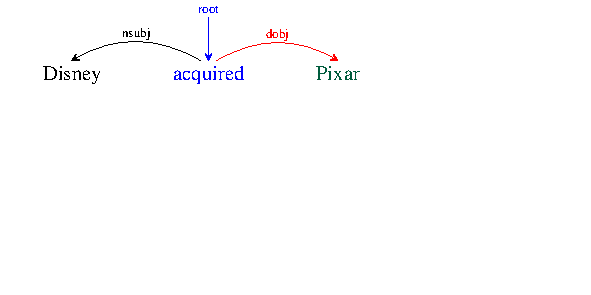
\includegraphics[trim=2em 9.4em 10em 0em,clip=true,scale=1.3]{figures/pixar_dobj}

\end{center}

\vspace{1cm}

\begin{block}{\centering Lambda Expression for dependency labels}
\vspace{-0.5cm}
\begin{align*}
  \hbox{\alert{dobj}} & \Rightarrow  \lambda \hlight{\mathbf{f}}\;\; \lambda {\color{blue!40!green!60!black} \mathbf{g}}\;\; \lambda \hlight{\mathbf{z}}\; \lspace \; \exists {\color{blue!40!green!60!black} \mathbf{x}}\; \lspace \; \hlight{\mathbf{f(z)}}\;\;\; \land \;\;\; {\color{blue!40!green!60!black} \mathbf{g(x)}}  \;\;\; \land\;\;\; \alert{\mathbf{arg_2}}(\hlight{\mathbf{z_e}}, {\color{blue!40!green!60!black} \mathbf{x_a}})
\end{align*}
\vspace{-0.5cm}
\end{block}
\end{frame}

\begin{frame}[noframenumbering]
\includegraphics[trim=1em 0em 0em 0em,clip=false,scale=1]{figures/dobj-lambda-calculus}
\end{frame} 

\subsection{DepLambda Composition}
\begin{frame}
\frametitle{Dependencies to Logical Forms}
\framesubtitle{Composition}
\begin{center}
\includegraphics[trim=2em 9.4em 10em 0em,clip=true,scale=1.3]{figures/pixar_dobj} 

\vspace{0.8cm}

\only<1>{\includegraphics[trim=7em 16em 7em 0em,clip=true,scale=1.1]{figures/dependency-transitive-derivation_dobj}\vspace{8em}}
\only<2>{\includegraphics[trim=7em 12em 7em 0em,clip=true,scale=1.1]{figures/dependency-transitive-derivation_dobj}\vspace{4em}}
\only<3>{\includegraphics[trim=7em 8em 7em 0em,clip=true,scale=1.1]{figures/dependency-transitive-derivation_dobj}}
\end{center}
\end{frame}

\begin{frame}
\frametitle{Dependencies to Logical Forms}
\framesubtitle{Composition}
\begin{center}
\only<1>{\includegraphics[trim=2em 9.4em 10em 0em,clip=true,scale=1.3]{figures/pixar_dobj_phrase}}
\only<2-4>{\includegraphics[trim=2em 9.4em 10em 0em,clip=true,scale=1.3]{figures/pixar_nsubj}}
\only<5->{\includegraphics[trim=2em 9.4em 10em 0em,clip=true,scale=1.3]{figures/pixar_nsubj_phrase}}

\vspace{0.8cm}

\only<1>{\hspace{1.2em}\includegraphics[trim=10em 16em 10em 0em,clip=true,scale=1.1]{figures/dependency-transitive-derivation-nsubj}\vspace{8em}}
\only<2>{\includegraphics[trim=3em 16em 3em 0em,clip=true,scale=1.1]{figures/dependency-transitive-derivation-nsubj}\vspace{8em}}
\only<3>{\includegraphics[trim=3em 12em 3em 0em,clip=true,scale=1.1]{figures/dependency-transitive-derivation-nsubj}\vspace{4em}}
\only<4>{\includegraphics[trim=3em 8em 3em 0em,clip=true,scale=1.1]{figures/dependency-transitive-derivation-nsubj}}
\only<5>{\includegraphics[trim=3em 8em 3em 0em,clip=true,scale=1.1]{figures/dependency-transitive-derivation_full}}
\end{center}
\end{frame}

\begin{frame}
\frametitle{Dependencies to Logical Forms}
 \vspace{0.6cm}
\begin{columns}
  \begin{column}{0.40\textwidth}
   \centering
  \vspace{-1em}
\includegraphics[trim=1.5em 9em 28em 0em,clip=true,scale=1.3]{figures/appos}   
  \end{column}
    \begin{column}{0.1\textwidth}
  \end{column}
  \begin{column}{0.58\textwidth}
    \large $\textsl{appos}  =$ \\ \hspace{0.5em} $ \lambda f \lambda g \lambda x \lspace f(x) \land g(x)$ \\
  \end{column}
 \end{columns}
 
 \pause
 \vspace{0.6cm}
 \begin{columns}
  \begin{column}{0.39\textwidth}
   \centering
\includegraphics[trim=1.5em 9em 26em 0em,clip=true,scale=1.2]{figures/partmod}
  \end{column}
  \begin{column}{0.1\textwidth}
  \end{column}
  \begin{column}{0.59\textwidth}
\large    $\textsl{partmod}= $ \\ \hspace{0.5em} $\lambda f \lambda g \lambda x \lspace \exists z \lspace f(x) \land g(z) \land \hbox{arg}_2(z_e, x_a)$ 
  \end{column}
  
 \end{columns}
 
 \pause
  \vspace{0.6cm}
 \begin{columns}
  \begin{column}{0.39\textwidth}
   \centering
\includegraphics[trim=1em 9em 28em 0em,clip=true,scale=1.3]{figures/conj}   
  \end{column}
  \begin{column}{0.1\textwidth}
  \end{column}
  \begin{column}{0.61\textwidth}
\large    $\textsl{conj} =$ \\ $ \lambda f \lambda g \lambda z \lspace \exists x y \lspace f(x) \land g(y) \land \mathrm{coord}(z,x,y)$ 
  \end{column}
 \end{columns}
\end{frame}

\begin{frame}
\frametitle{DepLambda}
\vspace{-2em}
\begin{center}
\includegraphics[trim=2em 7em 13em 0em,clip=true,scale=0.9]{figures/dependency-reduced-relative-ud}

\tikz[remember picture] \node[coordinate] (n1) {};\\
\vspace{2em}
\tikz[remember picture] \node[coordinate] (n2) {};

\begin{tikzpicture}[remember picture,overlay]   %% use here too
  \draw [->,>=stealth,shorten >=1pt,blue!20!white,line width=3pt] (n1) -- node[xshift=6em,black] {\footnotesize $\ldots >$ dobj $> \dots >$  nsubj $> \ldots$ } (n2);
\end{tikzpicture}

\includegraphics[trim=1em 47em 1em 0em,clip=true,scale=0.62]{figures/dependency-reduced-relative-derivation-ud}

\vspace{-1em}
\tikz[remember picture] \node[coordinate] (n3) {};\\
\vspace{2em}
\tikz[remember picture] \node[coordinate] (n4) {};

\begin{tikzpicture}[remember picture,overlay]   %% use here too
  \draw [->,>=stealth,shorten >=1pt,blue!20!white,line width=3pt] (n3) -- node[xshift=7em,black] {\footnotesize lambda expression composition} (n4);
\end{tikzpicture}

\vspace{-1em}
$\exists z. \mathrm{company(Pixar)} \wedge \mathrm{located}(z_e) \wedge \mathrm{arg_2}(z_e, \mathrm{Pixar}) \wedge \mathrm{arg_{in}}(z_e, \mathrm{CA})$
\end{center} 
\end{frame}

\begin{frame}
\frametitle{DepLambda in a nutshell}
\large

Dependency tree is a series of \hlight{compositions}

\vspace{2em}
Dependency label defines the \hlight{composition function}

\vspace{2em}
Each function takes two \hlight{typed}-semantic sub-expressions

\vspace{2em}
Returns typed-semantics of the larger expression
\end{frame}

\begin{frame}
\Large
\centering
\vspace{1.5em}
Freebase Semantic Parsing using DepLambda
\end{frame}

\section{Semantic Parsing as Graph Matching}
\begin{frame}
\frametitle{Freebase Semantic Parsing}
\framesubtitle{[Berant et al., 2013, Kwiatkowski et al., 2013]}
\vspace{-1em}
\begin{columns}
 \begin{column}{0.55\textwidth}
 %\vspace{-1cm}
 \begin{figure}
\begin{tikzpicture}[
  font=\sffamily,
  every matrix/.style={ampersand replacement=\&,column sep=0.2cm,row sep=1cm},
  myboxNL/.style={draw,thick,rounded corners,text width=15em,inner sep=0.15cm,fill=green!10},
  myboxMR/.style={draw,rounded corners,text width=15em,inner 
  sep=0.05cm,fill=red!5,draw=red!10}, 
  myboxAns/.style={draw,thick,rounded
  corners,text width=15em,inner sep=0.15cm,fill=yellow!10}, myArrow/.style={->,>=stealth,shorten >=1pt,blue!20!white,sloped,line width=10pt},
  myArrow1/.style={->,>=stealth,shorten >=1pt,blue!20!white,above,sloped,line width=10pt},
  every node/.style={align=center}]
\matrix{
    \node[myboxNL] (NL) {\textbf{Question} \\ Who is the director of Titanic?}; \\ 
    \only<2->{\node[myboxMR] (MR) [text=black!16] {
    \textbf{Grounded Logical Form} \\ $\lambda x.\exists e.\;\mbox{film.director}(x) \wedge \mbox{film.directed\_by}(e) \wedge \mbox{arg2}(y,x) \wedge \mbox{arg1}(e,\mbox{Titanic})$ }; \\}
    \node[myboxAns] (Ans) {\textbf{Answer} \\ \{James Cameron\}}; \\
    };
\end{tikzpicture}

\only<2->{\begin{tikzpicture}[rounded corners]

 \node[text width=15em,fill=white!0,draw=white!0](q_A) at (-5,-5) [text=red!80]{
\vspace{-4.2cm} \\ \hspace{2cm} Latent
 };
\end{tikzpicture}}
\end{figure}
 \end{column}

 \begin{column}{0.45\textwidth}
 \vspace{-1cm}
 \begin{figure}
  \includegraphics[scale=0.45]{figures/titanic} 
 \end{figure}
 \end{column}
\end{columns}
\end{frame}

\begin{frame}
\frametitle{End-to-End Semantic Parsing}
\framesubtitle{\scriptsize [Zelle \& Mooney, 1996; Zettlemoyer \& Collins, 2005; Kwiatkowski et al., 2010; Liang et al., 2011; \\
Artzi \& Zettlemoyer, 2011; Krishnamurthy \& Mitchell, 2012; Berant et al., 2013; Pasupat \& Liang, 2015; \\
Yih et al., 2015]}

\begin{columns}
 \begin{column}{0.5\textwidth}
 \large
  Grammar learning problem
  \visible<2->{
  \begin{itemize} \footnotesize
  \vspace{1em}
  \item director $\rightarrow$ $N: \lambda x \lspace \mbox{film.director}(x)$

  \vspace{1em}
  \item of $\rightarrow$ $(NP \backslash NP)/NP:$ $\lambda f 
  \lambda g \lambda x. \exists y\exists e \lspace f(y) \wedge g(x) \wedge \mbox{film.directed\_by}(e) \wedge $ $\mbox{arg1}(e, y) \wedge \mbox{arg2}(e,x)$
 \end{itemize}
}
 \end{column}
 \begin{column}{0.45\textwidth}
  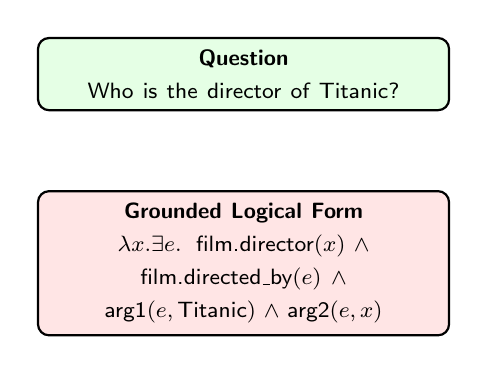
\begin{tikzpicture}[
  font=\sffamily,
  every matrix/.style={ampersand replacement=\&,column sep=0.2cm,row sep=1cm},
  myboxNL/.style={draw,thick,rounded corners,text width=14em,inner sep=0.15cm,fill=green!10},
  myboxMR/.style={draw,thick,rounded corners,text width=14em,inner sep=0.15cm,fill=red!10},
  myboxAns/.style={draw,thick,rounded corners,text width=14em,inner sep=0.15cm,fill=yellow!10},
  myArrow/.style={->,>=stealth,shorten >=1pt,blue!20!white,sloped,line width=10pt},
  myArrow1/.style={->,>=stealth,shorten >=1pt,blue!20!white,above,sloped,line width=10pt},
  every node/.style={align=center}]
\matrix{ 
    \node[myboxNL] (NL) {\footnotesize \textbf{Question} \\ \centering \footnotesize Who is the director of Titanic?}; \\
    \node[myboxMR] (MR) {\footnotesize \textbf{Grounded Logical Form} \\ \centering \footnotesize $\lambda x.\exists e.\;\mbox{film.director}(x) \wedge \mbox{film.directed\_by}(e) \wedge \mbox{arg1}(e,\mbox{Titanic}) \wedge \mbox{arg2}(e,x)$ }; \\
    % \node[myboxAns] (Ans) {\{oklahoma city, little rock, baton rouge, santa fe\}}; \\
    };
\end{tikzpicture}
 \end{column}
\end{columns}
\end{frame} 

\begin{frame}
\frametitle{Intermediate Semantic Parsing}
\framesubtitle{\scriptsize [Kwiatkowski et al., 2013;  Reddy et al., 2014; Choi et al., 2015; Artzi et al., 2015]}
 
\begin{columns}
 \begin{column}{0.5\textwidth}
 \large
 %\item Factorizes the problem into two.
 Language to \\ \hlight{ungrounded} logical form
 %\begin{itemize}
 %\item could exploit existing language processing tools
 %\item focus on the language aspect
 %\end{itemize}
 \vspace{2em} \\
 
 Ungrounded logical form to \hlight{grounded} logical form
 % \begin{itemize}
 % \item Exploit structural similarities
 % \item Powerful graph algorithms
 % \end{itemize} 
 \end{column}
 \begin{column}{0.45\textwidth}
  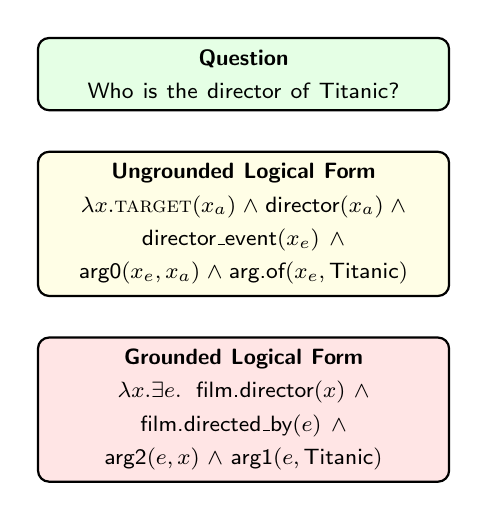
\begin{tikzpicture}[
  font=\sffamily,
  every matrix/.style={ampersand replacement=\&,column sep=0.2cm,row sep=0.5cm},
  myboxNL/.style={draw,thick,rounded corners,text width=14em,inner sep=0.15cm,fill=green!10},
  myboxMR/.style={draw,thick,rounded corners,text width=14em,inner sep=0.15cm,fill=red!10},
  myboxAns/.style={draw,thick,rounded corners,text width=14em,inner sep=0.15cm,fill=yellow!10},
  myArrow/.style={->,>=stealth,shorten >=1pt,blue!20!white,sloped,line width=10pt},
  myArrow1/.style={->,>=stealth,shorten >=1pt,blue!20!white,above,sloped,line width=10pt},
  every node/.style={align=center}]
\matrix{ 
    \node[myboxNL] (NL) {\footnotesize \textbf{Question} \\ \centering \footnotesize Who is the director of Titanic?}; \\
    \node[myboxAns] (MR) {\footnotesize \textbf{Ungrounded Logical Form} \\ \centering \footnotesize $\lambda x.\textsc{target}(x_a)\wedge \mbox{director}(x_a) \wedge\mbox{director\_event}(x_e) \wedge \mbox{arg0}(x_e,x_a) \wedge \mbox{arg.of}(x_e,\mbox{Titanic})$ }; \\
    \node[myboxMR] (MR) {\footnotesize \textbf{Grounded Logical Form} \\ \centering \footnotesize $\lambda x.\exists e.\;\mbox{film.director}(x) \wedge \mbox{film.directed\_by}(e) \wedge \mbox{arg2}(e,x) \wedge \mbox{arg1}(e,\mbox{Titanic})$ }; \\
    % \node[myboxAns] (Ans) {\{oklahoma city, little rock, baton rouge, santa fe\}}; \\
    };
\end{tikzpicture}
 \end{column}
\end{columns}
\end{frame}

\begin{frame}
\frametitle{Freebase Semantic Parsing: Task Setting}
\large

\hlight{Training Data:} Question and Answer Pairs

\vspace{2em}
\hlight{Evaluation:} Question Answering on Freebase

\vspace{2em}
\hlight{Resources:} Dependency Parser, DepLambda

\vspace{2em}
\hlight{Hypothesis}: DepLambda logical forms are useful
\end{frame}

\begin{frame}
\frametitle{Freebase is a Graph}
\begin{center}
\only<1>{\includegraphics[scale=0.8]{figures/knowledge_graph}}
\only<2>{\includegraphics[scale=0.8]{figures/knowledge_graph0}}
\only<3>{\includegraphics[scale=0.8]{figures/knowledge_graph1}}
\only<4>{\includegraphics[scale=0.8]{figures/knowledge_graph2}}
%\only<5>{\includegraphics[scale=0.8]{figures/knowledge_graph3}}
\end{center}
\end{frame} 

\begin{frame}
  \frametitle{Our Approach}

\only<1>{\includegraphics[scale=0.85]{figures/outline1.pdf}} 
\only<2>{\includegraphics[scale=0.85]{figures/outline2.pdf}}
\only<3>{\includegraphics[scale=0.85]{figures/outline3.pdf}}
\only<4>{\includegraphics[scale=0.85]{figures/outline4.pdf}}
\only<5>{\includegraphics[scale=0.85]{figures/outline.pdf}}
\end{frame}


\begin{frame}
\frametitle{Logical Form to Ungrounded Graph}
\centering{
\begin{tikzpicture}[rounded corners]
 \node[text width=30em,scale=1,fill=green!10,draw=blue](q_A) at (0,0)
 {
 \only<1>{\begin{center} \vspace{-0.5cm} \textit{Cameron directed Titanic in 
1997} \\
 $\lambda e. \mathrm{directed.arg1}(e, \textrm{\color{red} Cameron}) \wedge
 \mathrm{directed.arg2}(e, \textrm{\color{red} Titanic}) \wedge 
\mathrm{directed.in}(e,
 \textrm{\color{red} 1997})$ \end{center}}
 \only<2>{\begin{center} \vspace{-0.5cm} \textit{Cameron directed Titanic in 
1997} \\
 $\lambda e. \mathrm{directed.arg1}({\color{red} \bf e}, \texttt{Cameron}) 
\wedge
 \mathrm{directed.arg2}({\color{red} \bf e}, \texttt{Titanic}) \wedge 
\mathrm{directed.in}({\color{red} \bf e},
 \texttt{1997})$ \end{center}}
 \only<3>{\begin{center} \vspace{-0.5cm} \textit{Cameron directed Titanic in 
1997} \\
 $\lambda e. \mathrm{\color{red} directed.arg1}(e, \texttt{Cameron}) \wedge
 \mathrm{\color{red} directed.arg2}(e, \texttt{Titanic}) \wedge 
\mathrm{\color{red} directed.in}(e,
 \texttt{1997})$ \end{center}}
 };
\end{tikzpicture}}

\vspace{-0.2cm}
\begin{figure}
\centering
\only<1>{\includegraphics[scale=1,trim=0 0cm 0 
0,clip]{figures/main_example1}} 
\only<2>{\includegraphics[scale=1,trim=0 0cm 0 0,clip]{figures/main_example2}}
\only<3>{\includegraphics[scale=1,trim=0 0cm 0 0,clip]{figures/main_example3}}
\end{figure}
\vspace{-1.5cm}
\end{frame}

\begin{frame}
\frametitle{Graph Matching}

%\begin{figure}[t]
%\captionsetup[subfigure]{labelformat=empty}
%\vspace{-0.3cm}
%\subfloat[sub-caption][\color{blue} \scriptsize{Ungrounded graph}]{
\centering{
\only<1>{\includegraphics[scale=1]{figures/graph_pair1}}
\only<2>{\includegraphics[scale=1]{figures/graph_pair2}}
\only<3>{\includegraphics[scale=1]{figures/graph_pair3}}
}
 
\only<1,2,3>{{Ungrounded Graph \hspace{3cm} Grounded Graph}}
\end{frame}


\begin{frame}
  \frametitle{Graph Mismatch} 
  \large
  \centering
  What is the name of the director of Titanic?
  \vspace{1em}
  \begin{columns}
  \begin{column}{0.58\textwidth}
   \centering
   \only<1>{\includegraphics[width=\textwidth]{figures/transitive_ungrounded_mismatch} \\}
   \only<2>{\includegraphics[width=\textwidth]{figures/transitive_ungrounded_mismatch1} \\}
   \only<3>{\includegraphics[width=\textwidth]{figures/transitive_ungrounded_mismatch2} \\}
  \only<4>{\includegraphics[width=\textwidth]{figures/transitive_ungrounded_mismatch_collapsed} \\}
   Ungrounded graph
  \end{column}
  \begin{column}{0.42\textwidth}
    \centering
    \vspace{-1em}
   \includegraphics[width=\textwidth]{figures/transitive_grounded} \\
   \vspace{-1.5em}Grounded graph 
  \end{column}
 \end{columns}
 
 
 \only<3>{
   \vspace{2em}
 \begin{itemize}
   \item Paraphrasing is an alternative$^\dagger$\blfootnote{\scriptsize $^\dagger$Narayan, Reddy, Cohen (INLG 2016)}
 \end{itemize}
 \vspace{-5em}}
\end{frame}

\begin{frame}
\frametitle{Learning Model}
\large

\hlight{Structured Perceptron:} Ranks grounded and ungrounded graph pairs 
\only<1>{\includegraphics{figures/perceptron1}}
\only<2>{\includegraphics{figures/perceptron2}}
\only<3>{\includegraphics{figures/perceptron3}}
\only<4>{\includegraphics{figures/perceptron4}}
\only<5->{\includegraphics{figures/perceptron5}}

\vspace{0.5cm}



\visible<6->{\hlight{Training:} Use gold graph to update weights 
$$\theta \leftarrow \theta +
\Phi(g^+,u^+,q,\mathit{KB})\hspace{-.3ex}-\hspace{-.3ex}\Phi(\hat{g},\hat{u},q,\mathit{KB})$$}
\end{frame}

\begin{frame}
\frametitle{Learning Model}
\large 

\begin{itemize}
 \item[\huge $\star$] We \hlight{do not} have access to gold graphs
 \item[\huge $\star$] Access only to the \hlight{answers} rather than the query
 \item[\huge $\star$] Solution: use a \hlight{surrogate} gold graph
\end{itemize}

%\hlight{Oracle Graphs: } 
%\begin{itemize}
% \item[] Get grounded graphs matching an ungrounded graph
% \item[] Pick the graphs with minimal $F_1$-loss against the gold answer
%\end{itemize}

\pause
\vspace{0.5cm}
\hlight{Surrogate Gold Graph: }
\includegraphics{figures/perceptron-oracle}

%\vspace{0.5cm}
%\hlight{Beam Search: } Limit the predictions to~100 graph pairs
\end{frame}

\begin{frame}
\frametitle{Experimental Setup: UD}
\large
69 lambda calculus formulae

\vspace{2em}
WebQuestions in English, German, and Spanish

\vspace{2em}
BiLSTM Parser {\small [Kipperwiser and Goldberg (2016)]}\\
\begin{itemize}
\item English: 81.73 \\
\item German: 79.13 \\
\item Spanish: 85.76 \\
\end{itemize}
\end{frame}

\begin{frame}
\large
\frametitle{Baselines}
\hlight{$\underset{\mathrm{bag\; of\; words}}{\simplegraph:}$ }All entities connected to a single event
%\begin{itemize}
 % \item Does not handle compositional questions% in addition to a \textsc{target} node.
%\end{itemize}

% \pause

%\vspace{2em} 
% \hlight{\ccggraph: } CCG logical forms 

%\pause
\vspace{2em}
\hlight{\deptree:} Transduce a dependency tree to target graph \\
%An event for each head. Each dependent is linked to the event via its dependency relation. %Head is linked to the event via \textit{arg0}.

\end{frame}

\begin{frame}
\frametitle{Results on Multilingual WebQuestions}
\framesubtitle{English}
\centering
\large
\vspace{0.4em}
\includegraphics[trim=9.5em 0em 23em 0.5em,clip=true,scale=0.5]{figures/deplambda_results_plot_ud}
\end{frame}

\begin{frame}
\frametitle{Results on Multilingual WebQuestions}
\framesubtitle{German}
\centering
\large
\vspace{0.4em}
\includegraphics[trim=9.5em 0em 23em 0.5em,clip=true,scale=0.5]{figures/deplambda_results_plot_ud-de}
\end{frame}

\begin{frame}
\frametitle{Results on Multilingual WebQuestions}
\framesubtitle{Spanish}
\centering
\large
\vspace{0.4em}
\includegraphics[trim=9.5em 0em 23em 0.5em,clip=true,scale=0.5]{figures/deplambda_results_plot_ud-es}
\end{frame}

\begin{frame}
\frametitle{Experimental Setup: Stanford Dependencies} 
\large
78 lambda calculus formulae 

\vspace{2em}
Hypergraph parser {[\small Zhang \& McDonald (2014)]}
\begin{itemize}
\item English: 90.64
\end{itemize}

\vspace{2em}
Additional Baseline: 
\ccggraph \; -- CCG logical forms
\end{frame}

\begin{frame}
\frametitle{Results on WebQuestions}
%\centering
%\vspace{0.6em}
\only<1>{\includegraphics[trim=1em 12em 49.5em 0.5em,clip=true,scale=0.52]{figures/deplambda_results_plot}}
\only<2>{\includegraphics[trim=1em 12em 45em 0.5em,clip=true,scale=0.52]{figures/deplambda_results_plot}}
\only<3>{\includegraphics[trim=1em 12em 41em 0.5em,clip=true,scale=0.52]{figures/deplambda_results_plot}}
\only<4>{\includegraphics[trim=1em 12em 37em 0.5em,clip=true,scale=0.52]{figures/deplambda_results_plot}}
\only<5>{\includegraphics[trim=1em 12em 33em 0.5em,clip=true,scale=0.52]{figures/deplambda_results_plot}}
\only<6>{\includegraphics[trim=1em 12em 28em 0.5em,clip=true,scale=0.52]{figures/deplambda_results_plot}} 
\end{frame}

\section{Evaluation} 

\begin{frame}
\frametitle{Error Analysis}
\large
 \ccggraph fails to produce logical forms for 4.5\%.
 \begin{itemize}
  \item Sensitive to grammatical errors
  \item e.g., \textsl{what nestle owns?}
 \end{itemize}  
 
 \vspace{2em}
 DepLambda fails only for 0.9\%
 \begin{itemize}
   \item e.g., \textsl{what to do washington december}
 \end{itemize}  
\end{frame}

\begin{frame}  
\frametitle{Comparison with CCG}
\centering
\includegraphics[trim=0em 1em 1em 0em,clip=true,scale=1.2]{figures/ccg-transitive}
\end{frame}

\begin{frame}
\frametitle{Comparison with CCG}
\large
\vspace{-1em}
\begin{center}
\begin{tabular}{p{5.6cm}|p{5.6cm}}
 \multicolumn{1}{c|}{\hlight{CCG}} & \multicolumn{1}{c}{\hlight{DepLambda}} \\
 \midrule
 Lexicalized semantics & Simple lexical semantics \\
 \scriptsize $\hbox{S} \backslash \hbox{NP}/ \hbox{NP} : \lambda y \lambda x \lambda e \lspace \mathrm{acquired}(e) \land \mathrm{arg_1}(e, x) \land \mathrm{arg_2}(e, y)$  & \scriptsize $\lx \lspace \mathrm{acquired}(x_e)$ \\ 
\\
 Words drive composition & Dependencies drive composition \\
\\
 Language specific types & Mostly universal \\
 
%Argument adjunct distinction  & Every dependent is an adjunct \\
% \scriptsize $S\backslash NP/PP/NP$ vs. $(S\backslash NP)\backslash(S\backslash NP)/NP$ & \\
% Language specific categories & Mostly universal \\
%With ``complex~types'' comes power & Single-type system is robust, but restricted \\
%\scriptsize $(NP_{\hlight{\bf x}}\backslash NP_\hlight{\bf x})/(S\backslash NP_{\hlight{\bf x}})$ & \small $\lambda fgx \ldots $ i.e., $\eta \rightarrow \eta \rightarrow \eta$ for all labels \\
\end{tabular}
\end{center}
% \item Robust and no type checking necessary (a boon and a curse)
\end{frame}


\begin{frame}  
\frametitle{Comparison with CCG}
\centering
\includegraphics[trim=3em 1em 3em 0em,clip=true,scale=1.3]{figures/ccg-transitive-svo-derivation-tensors} 
\end{frame}

\begin{frame}
  \frametitle{DepLambda: \only<1,3,5>{\alert{Present}} \only<2,4,6>{\color{darkgreen}Towards ...}}
\large
Compositional Typed Semantics using Lambda Calculus \\
\pause
\includegraphics[trim=16em 14em 4em 10em,clip=true,scale=0.2]{figures/bullet}\; Richer composition functions e.g. neural networks

\vspace{2em}
\pause
Two universal types\\
\pause
\includegraphics[trim=16em 14em 4em 10em,clip=true,scale=0.2]{figures/bullet}\; Richer universal types

\pause
\vspace{2em}
Output: General-purpose logical forms\\
\pause \includegraphics[trim=16em 14em 4em 10em,clip=true,scale=0.2]{figures/bullet}\; Any target representation
\end{frame}

\section{Distantly-supervised Freebase Semantic Parsing}
\begin{frame}
\frametitle{This Talk}
\large 
\begin{enumerate}
 \item Dependencies to Logical Forms $\checkmark$
 
 \vspace{2em}
 \item Freebase Semantic Parsing using Logical Forms $\checkmark$
 
 \vspace{2em}
 \item Exploiting Text for Freebase Semantic Parsing
\end{enumerate}
\end{frame}

\begin{frame}
\Large
\centering
\vspace{1.5em}
\begin{enumerate}
 \setcounter{enumi}{2}
 \item Exploiting Text for Freebase Semantic Parsing \blfootnote{\color{blue} 
   $\bullet$ Xu, Reddy, Feng, Huang, Zhao (ACL 2016) \\
   \hspace{1.6em} $\bullet$ Bisk, Reddy, Blitzer, Hockenmaier (EMNLP 2016) \\
   \hspace{1.6em} $\bullet$ Reddy, Lapata, Steedman (TACL 2014)}
\end{enumerate}
\end{frame}

\section{Summary}
\begin{frame}
\frametitle{Summary}
\large


Compositional Typed Semantic interface for Dependencies
 
\vspace{2em} 
Dependencies to Logical Forms

 \vspace{2em}
Freebase Semantic Parsing using Logical Forms

\vspace{2em}
\begin{center}Demo at\\ \hlight{\url{https://sivareddy.in/deplambda.html}} \\
  Thank You!
\end{center}
\end{frame}

\begin{frame}
\frametitle{Semantic Parsing without QA pairs}
\vspace{-1em}
\begin{columns}
  \begin{column}{0.05\textwidth}
  \end{column}
 \begin{column}{0.55\textwidth}
  \only<1>{\includegraphics{figures/freebase_qa_pair}}
  \only<2>{\hspace{1em}\includegraphics{figures/freebase_qa_pair_striked}}
 \end{column}

 \begin{column}{0.45\textwidth}
 \vspace{-0.5cm}
 \begin{figure}
  \includegraphics[scale=0.45]{figures/titanic} 
 \end{figure}
 \end{column}
\end{columns}
\end{frame}

\begin{frame}
\frametitle{Semantic Parsing without QA pairs}

\begin{columns}
 \begin{column}{0.56\textwidth}
 \vspace{-1em}
 \begin{figure}
  \begin{tikzpicture}[
  font=\sffamily,
  every matrix/.style={ampersand replacement=\&,column sep=0.2cm,row sep=2cm},
  myboxNL/.style={draw,thick,rounded corners,text width=17em,inner sep=0cm,fill=green!10},
  myboxMR/.style={draw,thick,rounded corners,text width=17em,inner sep=0cm,fill=red!10},
  myboxAns/.style={draw,thick,rounded corners,text width=17em,inner sep=0.15cm,fill=yellow!10},
  myArrow/.style={->,>=stealth,shorten >=1pt,blue!20!white,sloped,line width=10pt},
  myArrow1/.style={->,>=stealth,shorten >=1pt,blue!20!white,above,sloped,line width=10pt},
  every node/.style={align=center}]
\matrix{
    \visible<1->{\node[myboxNL] (NL) {\begin{tabular}{l
    p{4.5cm}}\rotatebox[origin=c]{90}{\hspace{-1cm} \small \bf NL\phantom{xx}}
    & \small Leonardo DiCaprio starred as Jack in Titanic which was directed by James Cameron.
\\
\end{tabular}};} \\
    \visible<1->{\node[myboxMR] (MR) {\begin{tabular}{l
    p{4.6cm}}\rotatebox[origin=c]{90}{\hspace{-0.5cm} \small \bf KB\phantom{x}}
    & \small $\mbox{cast}(\textsc{Titanic},\textsc{DiCaprio},\textsc{Jack})
    \wedge\mbox{director}(\textsc{Titanic},\textsc{Cameron})$ \\
    \end{tabular}};}\\
\visible<1->{\node[myboxAns] (Ans) {\small \textsc{True}}; \\}\\
    };
    \visible<1->{\draw [myArrow] (NL) edge node[black] {Parser}  (MR);}
    \visible<1->{\draw [myArrow1] (MR) edge node[black]
    {\includegraphics[scale=0.2,angle=90]{figures/db}\\\vspace{-0.38cm}Execute} 
    (Ans);}
\end{tikzpicture}
\end{figure}
\end{column}

 \begin{column}{0.45\textwidth}
 \vspace{-3cm}
 \begin{figure}
  \includegraphics[scale=0.45]{figures/titanic} 
 \end{figure}
 \end{column}
\end{columns}
\end{frame}

\begin{frame}
 \frametitle{Task Setup}
 \large
 
 \hlight{Training Data:} Web Corpus
 
 \vspace{2em}
 \hlight{Evaluation:} Question Answering on Freebase
 
 \vspace{2em}
 \hlight{Resources:} Ungrounded Logical Forms
 
 \vspace{2em}
 \hlight{Hypothesis:} We do not need \hlight{manual} question answer pairs
\end{frame}


\begin{frame}
\frametitle{Learning from Text}
%unique

\begin{center}
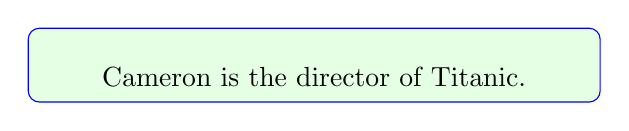
\begin{tikzpicture}[rounded corners]
 \node[text width=20em,scale=1,fill=green!10,draw=blue](q_A) at (0,0)
 {\begin{center} \raisebox{.5ex}[0pt]{Cameron is the director of Titanic.}\end{center} };
\end{tikzpicture}

\vspace{.5cm}

                \includegraphics[scale=1.2]{figures/unique_example}

\end{center}
\end{frame}

%%%%%%%%%%%%%%%%%%%%%%%%%%%%%%%%%%%%%%%%%%%%%%%%%%%%%%%%%

\begin{frame}
\frametitle{Learning from Text}

%arrow 
 
\begin{center}
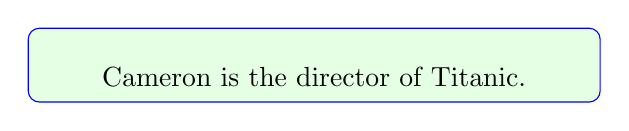
\begin{tikzpicture}[rounded corners]
 \node[text width=20em,scale=1,fill=green!10,draw=blue](q_A) at (0,0)
 {\begin{center} \raisebox{.5ex}[0pt]{\alert{Cameron} is the director of Titanic.}\end{center} };
\end{tikzpicture}

\vspace{.5cm}
                \includegraphics[scale=1.2]{figures/unique_example_query_pointed}

\vspace{.5cm}
Select one of the entities as target and replace it with~$x$ (here
\word{Cameron}). 
\end{center}
\end{frame}


%%%%%%%%%%%%%%%%%%%%%%%%%%%%%%%%%%%%%%%%%%%%%%%%%%%%%%%%%

\begin{frame}
\frametitle{Learning from Text}
% question-graph 1
\begin{center}
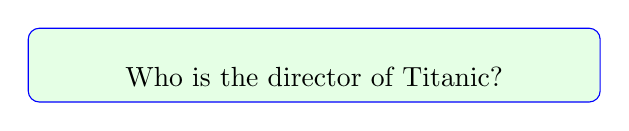
\begin{tikzpicture}[rounded corners]
 \node[text width=20em,scale=1,fill=green!10,draw=blue](q_A) at (0,0)
 {\begin{center} \raisebox{.5ex}[0pt]{\alert{Who} is the director of Titanic?}\end{center} };
\end{tikzpicture}

\vspace{.5cm}
             %   \color{blue!80} \scriptsize $\denot{x}{NL}$ = \{\textsc{Austin}\}
\includegraphics[scale=1.2]{figures/unique_example_query}\\

%                 $\denot{x}{NL}$ = \{\textsc{Austin}\}

\vspace{.5cm}
Build all knowledge base subgraphs with $x$ uninstantiated.
\end{center}
\end{frame}

%%%%%%%%%%%%%%%%%%%%%%%%%%%%%%%%%%%%%%%%%%%%%%%%%%%%%%%%%

\begin{frame}
\frametitle{Learning from Text}

\begin{center}
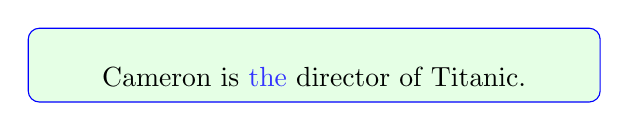
\begin{tikzpicture}[rounded corners]
 \node[text width=20em,scale=1,fill=green!10,draw=blue](q_A) at (0,0)
 {\begin{center} \raisebox{.5ex}[0pt]{\alert{Cameron} is \hlight{the} director of Titanic.}\end{center} };
\end{tikzpicture}


\vspace{.5cm}
                \includegraphics[scale=1.2]{figures/unique_example_query_pointed}\\
\vspace{.5cm}
\hlight{$\denot{x}{NL}$ = \{\textsc{Cameron}\}}
\vspace{.5cm}

Use denotations in NL and Freebase to select a surrogate gold graph. 
\end{center}
\end{frame}


%%%%%%%%%%%%%%%%%%%%%%%%%%%%%%%%%%%%%%%%%%%%%%%%%%%%%%%%%

\begin{frame}
\frametitle{Learning from Text}

\begin{center}
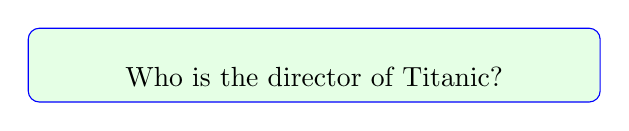
\begin{tikzpicture}[rounded corners]
 \node[text width=20em,scale=1,fill=green!10,draw=blue](q_A) at (0,0)
 {\begin{center} \raisebox{.5ex}[0pt]{\alert{Who} is the director of Titanic?}\end{center} };
\end{tikzpicture}

\vspace{.5cm}

\only<1>{
             %   \color{blue!80} \scriptsize $\denot{x}{NL}$ = \{\textsc{Austin}\}
\includegraphics[scale=.2]{figures/db} \includegraphics[scale=1.2]{figures/unique_example_grounded2}\\ 
           \hlight{$\denot{x}{KB}$ =
		\{\textsc{Cameron}, \textsc{JonLandau}\}}
	}
	
\only<2>{
             %   \color{blue!80} \scriptsize $\denot{x}{NL}$ = \{\textsc{Austin}\}
\includegraphics[scale=.2]{figures/db} \includegraphics[scale=1.2]{figures/unique_example_grounded2_wrong}\\ 
           \hlight{$\denot{x}{KB}$ =
		\{\textsc{Cameron}, \textsc{JonLandau}\}} \alert{$\neq$ $\denot{x}{NL}$}\\
	}
\vspace{.5cm}
Use denotations in NL and Freebase to select a surrogate gold graph. 

\end{center}

\end{frame}


%%%%%%%%%%%%%%%%%%%%%%%%%%%%%%%%%%%%%%%%%%%%%%%%%%%%%%%%%

\begin{frame}
\frametitle{Learning from Text}

\begin{center}
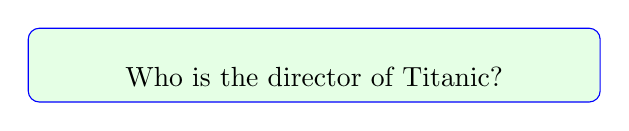
\begin{tikzpicture}[rounded corners]
 \node[text width=20em,scale=1,fill=green!10,draw=blue](q_A) at (0,0)
 {\begin{center} \raisebox{.5ex}[0pt]{\alert{Who} is the director of Titanic?}\end{center} };
\end{tikzpicture} 

\vspace{.5cm}

\only<1>{
\includegraphics[scale=.3]{figures/db} \includegraphics[scale=1.2]{figures/unique_example_grounded1}
\vspace{.5cm}

\hlight{$\denot{x}{KB}$ = \{\textsc{Cameron}\}}
}

\only<2>{
\includegraphics[scale=.3]{figures/db} \includegraphics[scale=1.2]{figures/unique_example_grounded1_correct} 
\vspace{.5cm}

\hlight{$\denot{x}{KB}$ = \{\textsc{Cameron}\} = $\denot{x}{NL}$}
}

\vspace{.5cm}
Use denotations in NL and Freebase to select a surrogate gold graph. 
\end{center}
\end{frame}
 
\begin{frame}
\frametitle{Learning from Text: Summary}
\large

\begin{itemize}
\item[] Learning proceeds by creating \alert{question-like graphs} by replacing named entities in logical forms mined from web
  text with a variable.

\vspace{2em}
  
\item[] Then try to find the subgraph of the knowledge graph with the
  the most \alert{similar denotation}.
\end{itemize}

\end{frame}

\begin{frame}
\frametitle{Results on \free}

\begin{table}
\begin{tabular}{|l| c c c c|}
  \hline
  System  & Precision & Recall & F1 &  \\
  \hline
  \textsc{mwg} & 52.6 & 49.1 & 50.8 & \\
   \kcaz & 72.6 & 66.1 & 69.2 & \\
   This Work  & \bf 81.9 & \bf  76.6 & \bf 79.2 & \color{blue} \bf +10.0 \\
   \hline
\end{tabular}
\end{table}

% \vspace{-0.5cm}
\begin{itemize}
  \item {\color{blue!70} \mwg:} Greedy Maximum Weighted Graph
  \item {\color{blue!70} \kcaz:} Kwiatkowski et al. 2013 
  \begin{itemize}
    \item Manually annotated QA pairs (612 pairs)
    \item Wiktionary
  \end{itemize}
\end{itemize}
\end{frame}

\begin{frame}
\frametitle{Results on \webq}
\begin{table}
\begin{tabular}{|l| c c c c c|}   
  \hline
  System  & Precision & Recall & F1 & $\underset{(\textsc{BL14})}{Avg F1}$ & \\
  \hline
  \textsc{mwg} & 39.4 & 34.0 & 36.5 & 41.6 & \\
  \textsc{BL14} & --- & --- & --- & 37.5 & \\
  This Work  & \bf 41.9 & \bf 37.0 & \bf 39.3 & \bf 47.7 &  \color{blue} \bf +10.2 \\
  \hline
\end{tabular}
\end{table}

%\vspace{0.5cm}

\begin{itemize}
  \setlength\itemsep{1em}
  \item {\color{blue!70} \mwg:} Greedy Maximum Weighted Graph
  
  \item {\color{blue!70} \textsc{BL14:}} Berant and Liang, 2014
  \begin{itemize}
    \item Manually annotated QA pairs (1115 pairs)
    \item Paraphrases and Web Corpus
  \end{itemize} 
\end{itemize}
\end{frame}


\section{Natural Logic for Semantic Parsing}
\begin{frame}
\frametitle{This Talk}
\large 
\begin{enumerate}
 \item Dependencies to Logical Forms $\checkmark$
 
 \vspace{2em}
 \item Freebase Semantic Parsing using Logical Forms $\checkmark$
 
 \vspace{2em}
 \item Exploiting Text for Freebase Semantic Parsing $\checkmark$
\end{enumerate}
\end{frame}

\begin{frame}
\Large
\vspace{1.5em}
QA without logical forms \blfootnote{\color{blue} 
  $\bullet$ Xu, Reddy, Feng, Huang, Zhao (ACL 2016)} \\
\end{frame}

\begin{frame}
\frametitle{Task Setting}
\large

\hlight{Training Data:} Question and Answer Pairs, Web Corpus

\vspace{2em}
\hlight{Evaluation:} Question Answering on Freebase

\vspace{2em}
\hlight{Resources:} Dependency Parser
\end{frame}


\begin{frame}
\frametitle{QA with Relation Extraction and Text Evidence}
\centering
\includegraphics[scale=0.8]{figures/natural-logic-flowchart}
\end{frame}

\begin{frame}
\frametitle{QA with Relation Extraction and Text Evidence}
\centering
\includegraphics[scale=0.7]{figures/natural-logic-argmax-flowchart}
\end{frame} 

\begin{frame}
\frametitle{QA with Relation Extraction and Text Evidence}
\includegraphics[trim=-12em 0em 0em 0em,clip=true,scale=0.7]{figures/natural-logic-argmax1}

\vspace{-4em}
\includegraphics[trim=-12em 0em 0em 0em,clip=true,scale=0.4]{figures/MCCNN}
\end{frame}

\section{Additional Slides}

\subsection{Motivation}
\begin{frame}
\frametitle{Syntax in humans?}
\begin{center}
\begin{columns}
\begin{column}{0.7\textwidth}
  \begin{quote}
   Studies on Peruvian Indian bilinguals indicate Quechua word order influences the local varieties of Spanish
   
   [Odlin, 1989]
  \end{quote}
\end{column}
\begin{column}{0.3\textwidth}
  \begin{center}
   \includegraphics[width=\textwidth]{figures/amazon-tribes}
  \end{center}
\end{column}
\end{columns}
\vspace{0.5cm}
\begin{columns}

\visible<2->{
\begin{column}{0.7\textwidth}
  \begin{quote}
   Arabs show strong preference for SVO in Dutch, whereas Turks for SOV
   
   [Jansen et al., 1981; Appel, 1984]
  \end{quote}
\end{column}
}
\begin{column}{0.3\textwidth}
   
\end{column}
\end{columns}
\end{center}
\end{frame}

\subsection{Single Type System}

\begin{frame}[noframenumbering]
\frametitle{Dependencies to Logical Forms}
\framesubtitle{Single Type System}
\vspace{-3em}
\begin{center}
\includegraphics[trim=2em 9.4em 10em 0em,clip=true,scale=1.3]{figures/pixar_dobj}

%\vspace{1cm}

%{({\color{red} dobj} {\color{blue} acquired} {\color{blue!40!green!60!black} Pixar})}
\end{center}

\vspace{1cm}

\begin{block}{\centering All constituents are of the same lambda expression type}
\centering
\vspace{0.1cm}
\type{{\color{blue} acquired}} =  \type{{\color{blue!40!green!60!black} Pixar}}  = \type{{({\color{red} dobj} {\color{blue} acquired} {\color{blue!40!green!60!black} Pixar})}}
\vspace{0.1cm}
\end{block}
\end{frame}

\begin{frame}[noframenumbering]
\frametitle{Dependencies to Logical Forms}
\framesubtitle{Single Type System}
\vspace{-0.8em}
\begin{center}
\includegraphics[trim=2em 9.4em 10em 0em,clip=true,scale=1.3]{figures/pixar_dobj}

%\vspace{1cm}

%{({\color{red} dobj} {\color{blue} acquired} {\color{blue!40!green!60!black} Pixar})}
\end{center}

\vspace{1cm}

\begin{block}{\only<1>{All \textbf{words} have a \textit{lambda expression} of type $\eta$}
\only<2->{All \textbf{constituents} have a \textit{lambda expression} of type $\eta$}}
\vspace{0.5em}
\begin{itemize}
  \item \type{{\color{blue} acquired}} = $\eta$
  \vspace{0.5em}
  \item \type{{\color{blue!40!green!60!black} Pixar}} = $\eta$
  \vspace{0.5em}
  \item<2-> \type{{({\color{red} dobj} {\color{blue} acquired} {\color{blue!40!green!60!black} Pixar})}} = $\eta$
  \vspace{1em}
\end{itemize}
\vspace{-0.3cm}
\visible<3->{$\implies$ \type{{\color{red} dobj}} = $\eta \rightarrow \eta \rightarrow \eta$}
\end{block}
\end{frame}

\begin{frame}[noframenumbering]
\frametitle{Dependencies to Logical Forms}
\framesubtitle{Lambda Calculus for Single Type System}
\vspace{-2.4em}
\begin{center}
\includegraphics[trim=2em 9.4em 10em 0em,clip=true,scale=1.3]{figures/pixar_dobj}

\end{center}

\vspace{1cm}

\begin{block}{Lambda Expression for words}
\vspace{-0.5cm}
\begin{align*}
  \hbox{\color{blue} acquired} & \Rightarrow  \lx_e \lspace \hbox{acquired}(x_e) & \visible<2->{\Rightarrow & \textbf{\textsc{type}} = \etype \rightarrow \btype} \\
  \hbox{\color{blue!40!green!60!black} Pixar} & \Rightarrow  \lx_a \lspace \hbox{Pixar}(x_a) &  \visible<2->{\Rightarrow & \textbf{\textsc{type}} = \itype \rightarrow \btype}
\end{align*}
\vspace{-0.5cm}
\end{block}
\visible<2->{Here \type{\hlight{acquired}} $\color{red} \neq$ \type{{\color{blue!40!green!60!black} Pixar}}  \alert \xmark}
\end{frame}

\begin{frame}
\frametitle{Dependencies to Logical Forms}
\framesubtitle{Lambda Calculus}
\vspace{-2.4em}
\begin{center}
\includegraphics[trim=2em 9.4em 10em 0em,clip=true,scale=1.3]{figures/pixar_dobj}

\end{center}

\vspace{1cm}

\begin{block}{\centering Lambda Expression for dependency labels}
\vspace{-0.5cm}
\begin{align*}
  \hbox{\alert{dobj}} & \Rightarrow  \lambda \hlight{\mathbf{f}}\;\; \lambda {\color{blue!40!green!60!black} \mathbf{g}}\;\; \lambda \hlight{\mathbf{z}}\; \lspace \; \exists {\color{blue!40!green!60!black} \mathbf{x}}\; \lspace \; \hlight{\mathbf{f(z)}}\;\;\; \land \;\;\; {\color{blue!40!green!60!black} \mathbf{g(x)}}  \;\;\; \land\;\;\; \alert{\mathbf{arg_2}}(\hlight{\mathbf{z_e}}, {\color{blue!40!green!60!black} \mathbf{x_a}})
\end{align*}
\vspace{-0.5cm}
\end{block}
\visible<2->{\hspace{3cm} This operation mirrors the tree structure}
\end{frame}

\begin{frame}[noframenumbering]
\frametitle{Dependencies to Logical Forms}
\framesubtitle{Lambda Calculus for Single Type System}
\vspace{-2.4em}
\begin{center}
\includegraphics[trim=2em 9.4em 10em 0em,clip=true,scale=1.3]{figures/pixar_dobj}
\end{center}

\vspace{1cm}

\begin{block}{Lambda Expression for words}
\vspace{-0.5cm}
\begin{align*}
  \hbox{\color{blue} acquired} & \Rightarrow  \lambda \mathbf{\color{red} x_a} x_e \lspace \hbox{acquired}(x_e) & \visible<2->{\Rightarrow & \textbf{\textsc{type}} = \ptype  \rightarrow \btype} \\
  \hbox{\color{blue!40!green!60!black} Pixar} & \Rightarrow  \lx_a {\mathbf{\color{red} x_e}} \lspace \hbox{Pixar}(x_a) &  \visible<2->{\Rightarrow & \textbf{\textsc{type}} = \ptype \rightarrow \btype}
\end{align*}
\vspace{-0.5cm}
\end{block}
\visible<2->{Here $\eta$ = \type{\hlight{acquired}} = \type{{\color{blue!40!green!60!black} Pixar}} $\hlight \checkmark$} 
\end{frame}

\subsection{Complex constructions}
\begin{frame}[noframenumbering]
\frametitle{Relative Clause in CCG}
\centering
\includegraphics[scale=0.7]{figures/ccg-relative-clause}
\end{frame}

\begin{frame}[noframenumbering]
\frametitle{Relative Clause in DepLambda}
\framesubtitle{following Carpenter (1998)}
\begin{center}
\includegraphics[trim=1em 7.5em 22em 0em,clip=true,scale=1]{figures/relative-object-extraction-ud}

\vspace{3em}

\includegraphics[trim=1em 6.5em 17em 0em,clip=true,scale=1]{figures/relative-object-extraction-binding-ud}

\ignore{
\begin{small}
\begin{tabular}{l}\\
  $\mathrm{(acl}$ \hspace{0.3cm}  $\mathrm{company}$ \\ 
  \hspace*{1cm} ($\hlight{\bind}$ $\alert{f}$ \\
  \hspace*{2cm}  $\mathrm{(wh}$-$\mathrm{dobj}$  \\  
  \hspace*{3cm} $\mathrm{(nsubj}$ \\
  \hspace*{4cm} $\mathrm{(dobj~acquired}$~$f)$\\
  \hspace*{3cm}$\mathrm{~Disney))}$ \\
  \hspace*{2cm} $\mathrm{which)))}$
\end{tabular}
\end{small}
}
\end{center}
\end{frame}

\begin{frame}[noframenumbering]
\frametitle{Comparison with CCG}

Handling of control verbs is painful.

\vspace{0.5cm}
\textbf{Sentence:}\\
\textsl{John persuaded Jim to acquire Pixar}.

\vspace{0.3cm}
\textbf{Binarized Tree:}\\
(nsubj (xcomp (dobj persuaded Jim) to\_acquire\_Pixar) John)

\pause
\vspace{0.3cm}
\textbf{Elegant handling in CCG} \\
\hspace{0.5cm} persuaded: $((S[dcl]\backslash NP)/(S[to]\backslash NP_{\hlight{x}}))/NP_{\hlight{x}}$
\end{frame}


\begin{frame}[noframenumbering]
\frametitle{Conjunctions}

\textbf{Sentence:} \\
{\centering Eminem signed to Interscope and discovered 50 Cent. \\} 

\vspace{0.3cm}  
\textbf{Binarized tree:} \\
{\centering (nsubj (conj-vp (cc s\_to\_I and) d\_50) Eminem) \\}

\pause
\vspace{0.3cm}  
\textbf{Substitution:} 

\begin{tabbing}
  conj-vp $\Rightarrow$ $\lambda f g x \lspace \exists y z \lspace f(y) \land g(z) \land \mathrm{\hlight{coord}}(x, y, z)$
\end{tabbing}

\vspace{0.3cm}  
\textbf{Logical Expression:}
\begin{tabbing}
  $\lambda w \lspace$\=$\exists x y z \lspace \mathrm{Eminem}(x_a) \land \mathrm{\hlight{coord}}(w, y, z)$ \\
\> $\land\, \mathrm{arg_1}(w_e, x_a) \land\, \mathrm{s\_to\_I}(y) \land \mathrm{d\_50}(z)$
\end{tabbing}

\pause
\textbf{Post processing:}
\begin{tabbing}
$\lambda e \lspace$\=$\exists x y z \lspace \mathrm{Eminem}(x_a) \land \mathrm{arg_1}(y_e, x_a)$ \\
\> $\land\,\mathrm{arg_1}(z_e, x_a) \land \mathrm{s\_to\_I}(y) \land \mathrm{d\_50}(z)$
\end{tabbing}
\end{frame}

\begin{frame}[noframenumbering]
\frametitle{Relative Clause}
\framesubtitle{following Moortgat (1988); Pereira (1990); Carpenter (1998)}
\textbf{Sentence:} \\
{\centering Apple which Jobs founded\\} 

\textbf{Binarized tree:} \\
\begin{small}
\begin{tabular}{l}\\
$\mathrm{(rcmod}$  $\mathrm{Apple}$ \\ 
  \hspace*{1cm} $\mathrm{(wh}$-$\mathrm{dobj}$
  ($\hlight{\bind}$ $f$ $\mathrm{(nsubj~(dobj~founded}$~$f$$\mathrm{)~Jobs))}$ \\
\hspace*{2.5cm} $\mathrm{which))}$
\end{tabular}
\end{small}

\pause
\textbf{Substitution:} 
\begin{tabbing}
wh-dobj $\Rightarrow$ $\lambda f g z \lspace f(z)$\\
rcmod $\Rightarrow$ $\lambda f g z \lspace f(z) \land g(z)$
\end{tabbing}

\textbf{Logical Expression:}
\begin{tabbing}
$\lambda u \lspace \exists x y \lspace$\=$\mathrm{founded}(x_e) \land \mathrm{Jobs}(y_a)$\\
\>$\land\, \mathrm{arg_1}(x_e, y_a)
\land \mathrm{arg_2}(x_e, u_a) \land \mathrm{Apple}(u_a)$
\end{tabbing}
\end{frame}

\begin{frame}[noframenumbering]
\frametitle{Expressivity}
How isomorphic are the representations compared to Knowledge Graph?

Average Oracle $F_1$ Table.

\end{frame}

\begin{frame}[noframenumbering]
\frametitle{Search Space}
How many ways to reach an answer? 

Average Oracle $F_1$ Table.

\end{frame}

\subsection{Graph Operations}
\begin{frame}[noframenumbering]
\frametitle{Graph Transformation: \contract operation}

\begin{center}
  What is the \hlight{name of the company} which Disney acquired in 2006?
\end{center}

\begin{columns}
  \begin{column}{0.35\textwidth}
   \centering
   \includegraphics[width=\textwidth]{figures/question_unmerged_ungrounded_graph} \\
   \small Ungrounded graph
  \end{column}
  \begin{column}{0.35\textwidth}
    \centering
   \includegraphics[width=\textwidth]{figures/question_merged_ungrounded_graph} \\
   \small Grounded graph 
  \end{column}
\end{columns}
\end{frame}

\begin{frame}[noframenumbering]
\frametitle{Graph Mismatch: \expand operation}

 %\item Due to parse errors, sometimes not all entities are in the ungrounded graph
 %\item \expand operator connect these entities to the main event
 What to do Washington DC December? \\
 

 \vspace{0.5cm} 
 \textbf{Before \expand}
 \begin{itemize}
   \item $\lambda z \lspace \exists x y w \lspace \textsc{target}(x_a) \land
\mathrm{do}(z_e) \land \mathrm{arg_1}(z_e, x_a) \land
\mathrm{Washington\_DC}(y_a) \land \mathrm{December}(w_a)$
   \end{itemize}
 
 \vspace{0.5cm}
 \textbf{After \expand}
 \begin{itemize}
   \item $\lambda z\lspace \exists x y w \lspace \textsc{target}(x_a) \land \mathrm{do}(z_e) \land \mathrm{arg_1}(z_e, x_a) \land \mathrm{Washington\_DC}(y_a) \land
   \mathrm{\hlight{dep}}(z_e, y_a) \land \mathrm{December}(w_a) \land \mathrm{\hlight{dep}}(z_e, w_a)$
   \end{itemize}
\end{frame}

\subsection{Semantic Parsing without QA Datasets}
\begin{frame}[noframenumbering]
\frametitle{Experiments}
 \hlight{Target Domains:}  Business, Film, People 
  \begin{itemize}
    \item Largest domains of Freebase
    \item 120m triples, 411 relations and 210 types.
  \end{itemize}
  
  \vspace{1em}
  \hlight{Training data:} 99K sentences from ClueWeb09
\end{frame}


\begin{frame}[noframenumbering]
\frametitle{Experiments}

  \hlight{Test data:} 
  \begin{itemize}
  	\item \free [Cai and Yates, 2013] 
  	\begin{itemize}
  	 \item Syntactically well-formed queries
  	 \item 124 queries for our target domains
  	\end{itemize}

  	\item \webq [Berant et al., 2013] 
  	\begin{itemize}
	  \item Google search queries starting with \textit{wh} question words.
	  \item 570 queries for our target domains
	\end{itemize}
  \end{itemize}
\end{frame}

\end{document}
